% 2022 University of Pennsylvania PhD Dissertation LaTeX Template v.20221216
% This template aims to fulfill University formatting requirements when one follows the instructions, resolves errors and warnings, and does not edit the style file or font size. Consult https://provost.upenn.edu/formatting-faqs for the most up-to-date requirements and policies.
%-------------------------------------------
% We welcome your feedback on the template https://upenn.libwizard.com/f/dissertationlatextemplatefeedback
%-------------------------------------------
% The template requires TeX Live 2022 and is optimized for pdfLaTeX and the LaTeX editor Overleaf. Other LaTeX editing programs may require you to compile the document more than once. It is adapted from the Penn Biostat LaTeX Template modified from Dissertation Template for Wharton PhD Candidates in LaTeX. Portions of the text are reprinted or adapted with permission from Ratcliffe SJ. (2017) Penn Biostat LaTeX Template: PhD dissertation. https://dbe.med.upenn.edu/biostat-research/Dissertation_template

%%%%%%%%%%%%%%%%%%%%%%%%%%%%%%%%%%%%%%%%%%%%%%%%
%%%%%%%%%%%%%%%%%%%%%%%%%%%%%%%%%%%%%%%%%%%%%%%%
\documentclass[11pt]{report}
\usepackage{upennstyle} % You may add additional packages below this line. Overleaf will warn you if your packages conflict with the template packages. See Chapter 1 for more information.

%-------------------------------------------
% Citation and bibliography commands. Edit as needed.
\usepackage[nonamebreak,round]{natbib}
\bibliographystyle{plainnat}
%-------------------------------------------

%%%%%%%%%%%%%%%%%%%%%%%%%%%%%%%%%%%%%%%%%%%%%%%%
%%%%%%%%%%%%%%%%%%%%%%%%%%%%%%%%%%%%%%%%%%%%%%%%
% PLEASE FOLLOW THE INSTRUCTIONS IN THE CODE COMMENTS
% To uncomment a line of code, remove the % at the beginning of the line
% To comment out a line of code, add a % at the beginning of the line
%%%%%%%%%%%%%%%%%%%%%%%%%%%%%%%%%%%%%%%%%%%%%%%%
%%%%%%%%%%%%%%%%%%%%%%%%%%%%%%%%%%%%%%%%%%%%%%%%

%%%%% PRELIMINARY PAGES %%%%%
%-------------------------------------------
%%%% TITLE PAGE
% Edit the text between curly braces {} relevant to your dissertation.
\title{Empirical Evidence That Using AI Tools Can Enhance Human Cognition}
\author{Benjamin Lira Luttges}
%\specialization{Field of Specialization} % If you are in Romance Languages or Managerial Science and Applied Economics (Wharton), uncomment this line and edit the text between the {}. If you do, you will also need to edit lines 71 and 72.
\gradgroup{Psychology} % See https://provost.upenn.edu/phd-graduate-groups for names
\date{2025} % Enter current four-digit year
\supervisor{Angela L. Duckworth}
\supervisortitle{Rosa Lee and Egbert Chang Professor}
%\cosupervisor{Co-supervisor's Typed Name} % If applicable, uncomment this line and edit the text between the {}. If you do, you will also need to edit line 39. 
%\cosupervisortitle{Full Faculty Title and Affiliation} % If applicable, uncomment this line and edit the text between the {}. If you do, you will also need to edit line 38.
\gradchair{Sara Jaffee, Professor of Psychology, University of Pennsylvania}
\committee{Lyle Ungar, Professor of Computer and Information Science, University of Pennsylvania}
\committee{Martin Seligman, Zellerbach Family Professor of Psychology, University of Pennsylvania}
% \committee{Committee Member's Typed Name, Full Faculty Title and Affiliation} % If applicable, comment out or duplicate this line to remove or add a committee member
%-------------------------------------------

%%%% OPTIONAL COPYRIGHT NOTICE
\authorlegal{Benjamin Lira Luttges} % To opt out of copyrighting your dissertation, uncomment this line. If you do, you will also need to edit line 76.
%-------------------------------------------
%\cclicense{Name of Selected Creative Commons License} % If applicable, uncomment this line and edit the text between the {}. If you do, you will also need to edit lines 51, 76, and 78.
%-------------------------------------------
%\cclicenseurl{URL of selected Creative Commons License} % If applicable, uncomment this line and edit the text between the {}. If you do, you will also need to edit lines 49, 76, and 78.
%-------------------------------------------

%%%% OPTIONAL DEDICATION
\dedication{Write your dedication text in italics here.} % If not applicable, comment out this line to hide the optional dedication page. If you do, you will also need to edit line 82.
%-------------------------------------------

%%%% OPTIONAL ACKNOWLEDGEMENT
\acknowledgement{Write your acknowledgement text here.} % If not applicable, comment out this line to hide the optional acknowledgement page. If you do, you will also need to edit line 86.
%-------------------------------------------

%%%% ABSTRACT
\abstract{Many worry that AI tools boost productivity in the short-term, at a long-term cost in the development of human capability. Using AI will rob us of the opportunity to learn, will destroy our motivation for hard work, and will perpetuate the biases in its training data. I propose two theoretically distinct mechanisms through which AI influences human cognition–engagement and information–and provide three empirical demonstrations of AI tools proving information (Chapters 1 and 3) and motivation (Chapter 2).

In Chapter 1, I show that superior information—in the form of just-in-time, personalized examples—can compensate for decreased engagement, yielding net positive effects on skill development. Participants writing cover letters with AI assistance improved more on writing tests than those practicing without AI, despite exerting less effort. A second experiment showed participants learned more from exposure to AI-generated examples even when they could not edit them. These gains were unique to AI, outperforming static online examples and matching feedback from professional editors.

In Chapter 2, I show that an AI chatbot can increase motivation among Khan Academy users. In this year-long field investigation, I built two AI-based chatbots that delivered situation modification and emotional reframing interventions. Relative to the week before exposure to the chatbots, students increased their time on task by 10-11\% and worked on more challenging problems after completing interventions.

Finally, in Chapter 3, I demonstrate the potential for AI to enhance human decision making in the high-stakes setting of college admissions. I fine-tuned a language model to assess personal qualities like leadership, training it on professional admissions officers' evaluations of 3,131 applicant essays. The AI successfully reproduced expert judgment, and did so equally well across demographic subgroups, showing no evidence of bias. Scaling its application to a national sample of 309,594 applicants revealed that these scores incrementally predicted graduation rates without encoding demographic information. This demonstrates that AI need not be a biased 'black box'—careful training can produce interpretable systems that enhance rather than distort human judgment.

Collectively, the chapters in this dissertation show that smarter machines do not inevitably produce stupider humans. AI tools, when carefully designed and deployed, can improve motivation and information processing, making us better writers, more motivated learners, and wiser decision makers.} % Write your abstract between the {}
%-------------------------------------------

%%%% OPTIONAL PREFACE
%\preface{Write your preface text here.} % If applicable, uncomment this line and write your preface between the {}. If you do, you will also need to edit line 101.
%-------------------------------------------

\begin{document}

\maketitle % If you are in Romance Languages or Managerial Science and Applied Economics (Wharton), comment out this line. If you do, you will also need to edit lines 33 and 72.
%\makespecializationtitle % If you are in Romance Languages or Managerial Science and Applied Economics (Wharton), uncomment this line. If you do, you will also need to edit lines 33 and 71.
\setcounter{page}{2}

%%%% OPTIONAL COPYRIGHT NOTICE
\makecopyright % If not applicable, comment out this line to hide the optional traditional copyright notice page. If you do, you will also need to edit line 47.
%-------------------------------------------
%\makecreativecommons % If applicable, uncomment this line to insert the optional Creative Commons License copyright notice page. If you do, you will also need to edit lines 49, 51, and 76.
%-------------------------------------------

%%%% OPTIONAL DEDICATION PAGE
% \makededication % If not applicable, comment out this line to hide the optional dedication page. If you do, you will also need to edit line 55.
%-------------------------------------------

%%%% OPTIONAL ACKNOWLEDGEMENT PAGE
% \makeacknowledgement % If not applicable, comment out this line to hide the optional acknowledgment page. If you do, you will also need to edit line 59.
%-------------------------------------------

\makeabstract
\tableofcontents

% %%%% OPTIONAL LIST OF TABLES
% \clearpage \phantomsection \addcontentsline{toc}{chapter}{LIST OF TABLES} \begin{singlespacing} \listoftables \end{singlespacing}% If not applicable, comment out this line to hide the optional List of Tables
% %-------------------------------------------

% %%%% OPTIONAL LIST OF ILLUSTRATIONS
% \clearpage \phantomsection \addcontentsline{toc}{chapter}{LIST OF ILLUSTRATIONS} \begin{singlespacing} \listoffigures \end{singlespacing}% If not applicable, comment out this line to hide the optional List of Illustrations
% %-------------------------------------------

%%%% OPTIONAL PREFACE
%\makepreface % If applicable, uncomment this line to insert the optional preface. If you do, you will also need to edit line 67.
%-------------------------------------------

%%%%% MAIN TEXT %%%%%
\begin{mainf} % The main body of your dissertation starts below this line

\chapter{Learning, not cheating: AI assistance can enhance rather than hinder skill development}

\section{Abstract}
Does using AI make you stupid? In particular, do the immediate productivity gains of outsourcing cognitive work to AI come at the expense of long-term human capital development? In this investigation, lay forecasters predicted that practicing writing cover letters with an AI tool would impair learning compared to practicing writing letters without the tool. However, in a pre-registered experiment, participants randomly assigned to practice writing with AI improved more on a writing test one day later compared to writers assigned to practice without AI. Notably, writers given access to the AI tool improved more despite exerting less effort, as measured by time on task, keystrokes, or subjective ratings. Similarly, lay forecasters predicted that AI tools would be less helpful, and less worth paying for, than feedback from experienced human editors. Contrary to this intuition, a second preregistered experiment showed that practicing writing with an AI tool improved writing skill more receiving personalized feedback from professional human editors. Finally, in a third pre-registered experiment, we tested the possibility that AI teaches by example: writers merely shown an AI-generated cover letter (without the opportunity to practice) performed as well as writers who practiced writing with the original AI tool. Collectively, these findings constitute an existence proof that by providing personalized and high-quality examples, AI tools can improve, rather than undermine, learning. \footnote{This work is currently under review at Science Advances} 

\section{Introduction}

Generative AI (henceforth AI) tools are increasingly powerful and prevalent \cite{bubeck2023}, and there is mounting evidence that they can dramatically boost performance. 
  For example, working side-by-side with AI as a copilot has been shown to increase both quality and speed in a variety of professional writing tasks (e.g., emails, memos, short reports) \cite{noy2023, dellacqua2023, wiles2023algorithmic}.

Nevertheless, there is growing concern that AI tools will be used as a crutch, providing immediate gains in performance at the expense of long-run development of human capital~\cite{hofman2023sports, puntoni2021, borges2024}.
  For instance, in a 2024 poll, 62\% of surveyed adults predicted that Generative AI will ``lead to humans becoming less intelligent'' \cite{hawkins2024between}.
  In January 2023, New York City public schools banned ChatGPT, citing ``concerns about negative impacts on student learning \cite{roose2023}.'' 
  When this ban was lifted three months later, it was not because of AI’s potential to scaffold learning, but instead because of the ``reality that students are participating in and will work in a world where understanding Generative AI is crucial \cite{banks2023}.'' 
  The sentiment behind the initial ban aligns with teacher perceptions: 
  in a nationally representative poll in May 2024, four times as many K-12 educators judged the use of AI tools as net harmful (24\%) than net beneficial (6\%) \cite{lin2024a}. 

Concerns that using AI tools hinders learning (while increasing short-term performance) are justified for at least three reasons. 
  First, AI systems based on large language models like GPT-4 have been shown to confidently assert erroneous facts (i.e., hallucinations \cite{ji2023survey}), make reasoning and arithmetic errors \cite{yuan2023well}, and complete other tasks with varying degrees of accuracy.
  
Second, regardless of accuracy, the fluent and instantaneous solutions AI tools generate may contribute to an illusion of mastery. 
  To the extent users conflate the skills of an AI tool with their own, they may be less likely to seek feedback and improve. 
  Prior research has found that searching for information on the Internet, for example, creates an illusion whereby people conflate knowledge outside their heads with what they personally know themselves \cite{fisher2015}.

Third, technological tools reduce the need for the learner to be cognitively engaged with the task at hand. 
  For instance, knowing that we will be able to search for a fact on a computer has been shown to reduce memory for that fact, instead encouraging recall of how to search for it \cite{sparrow2011}. 
  And drivers who use GPS tend to have worse hippocampal-dependent spatial memory, both cross-sectionally and longitudinally \cite{maguire2000, griesbauer2022london}. 
  To the extent that tools powered by generative AI instantaneously produce turn-key solutions for complex cognitive tasks, they may be especially detrimental to learning. 
  It is, after all, tempting to copy and paste the output of an AI tool without even laying eyes on it.  

And yet there is a plausible, albeit less obvious, alternate hypothesis: Using AI tools to help do our work could help us develop our own skills. 
    In particular, the current generation of AI tools may teach by example, offering high-quality and personally tailored demonstrations of abstract principles that are otherwise difficult to grasp and apply.
    Classic research shows that worked examples of math problems (i.e., not just answers but the step-by-step process by which problems are solved) scaffold learning more effectively than explanations alone \cite{sweller1985use, atkinson2000learning}. 
     Compared to textbooks, conventional computer tutoring programs (e.g., \cite{anderson1995cognitive}), and even human teachers, AI tools may be able to provide higher-quality, just-in-time examples exquisitely tailored to a learner's specific needs.  Indeed, it may be that in both quality and didactic utility, AI examples (e.g., of an excellent cover letter)  might surpass even those provided by domain experts (e.g., professional writers and editors).  
    Thus, AI tools may improve skill development if the upside of exposure to excellent examples tailored to the learners' needs outweighs the downside of diminished engagement. 

There is little research on how AI tools influence skill development. 
  In working papers, results have been mixed. 
  Some studies have found that interacting with AI tools improves skill on subsequent tests in which AI tools are not available \cite{kumar2023, lehmann2024ai}, while others have shown null or even negative effects \cite{bastani2024, nie2024gpt,lehmann2024ai}. 
  Notably, these studies examine AI tutors, chatbots, or explanations explicitly designed to support learning, rather than simply providing solutions as is typical in real-world use. 
  Further, they focus exclusively on mathematics and computer programming. 

In this investigation, we ask whether AI tools can increase intermediate-term skill development, above and beyond just improving performance while using the AI tool.
  We focus on writing---the most common use of AI at work, as ranked in a nationally representative survey of American adults in August 2024  \cite{bick2024rapid}. 
  Participants in our three pre-registered studies were American adults on the survey platform Prolific. 
  
  To differentiate the effects of AI use on learning versus performance, we developed a paradigm in which all participants were given a baseline writing test (i.e., revising a poorly written cover letter).
  They were then introduced to evidence-based strategies for professional writing, with descriptions and examples for each one \cite{rogers2023,shulman2024}. 
  Next, participants were randomly assigned to one of three conditions: practicing rewriting a different cover letter with access to an AI tool based on the same writing principles that users had just learned (See Figure \ref{fig:tool}), practicing without this tool, or a no-practice control group. 
  To assess gains in writing skill, participants completed an incentivized test in which they rewrote yet another cover letter without access to AI, with a cash bonus guaranteed for submissions ranked in the top 10 percent. 
  To assess the persistence of skill improvement, all participants were invited to complete a similar incentivized test of writing skill one day later.
  See Figure \ref{fig:design}.
  We used GPT4o to rate each cover letter for each of the five writing principles introduced in this experiment. We averaged these ratings to produce summary scores of writing skill and, in a random subsample (\textit{n} = 30), validated these scores using trained human raters (\textit{r} = .83, \textit{p} < .001).
  Additionally, we asked a separate sample of participants to read pairs of test-phase cover letters randomly selected from different conditions, and to indicate which letter would be more likely to secure a job interview. 
  Cover letters more likely to secure an interview obtained higher AI ratings of writing skill (\textit{r}s = .29 and .28, \textit{p}s < .001, for Study 2 and 3, respectively). 

\begin{figure*}[t]
    \centering
    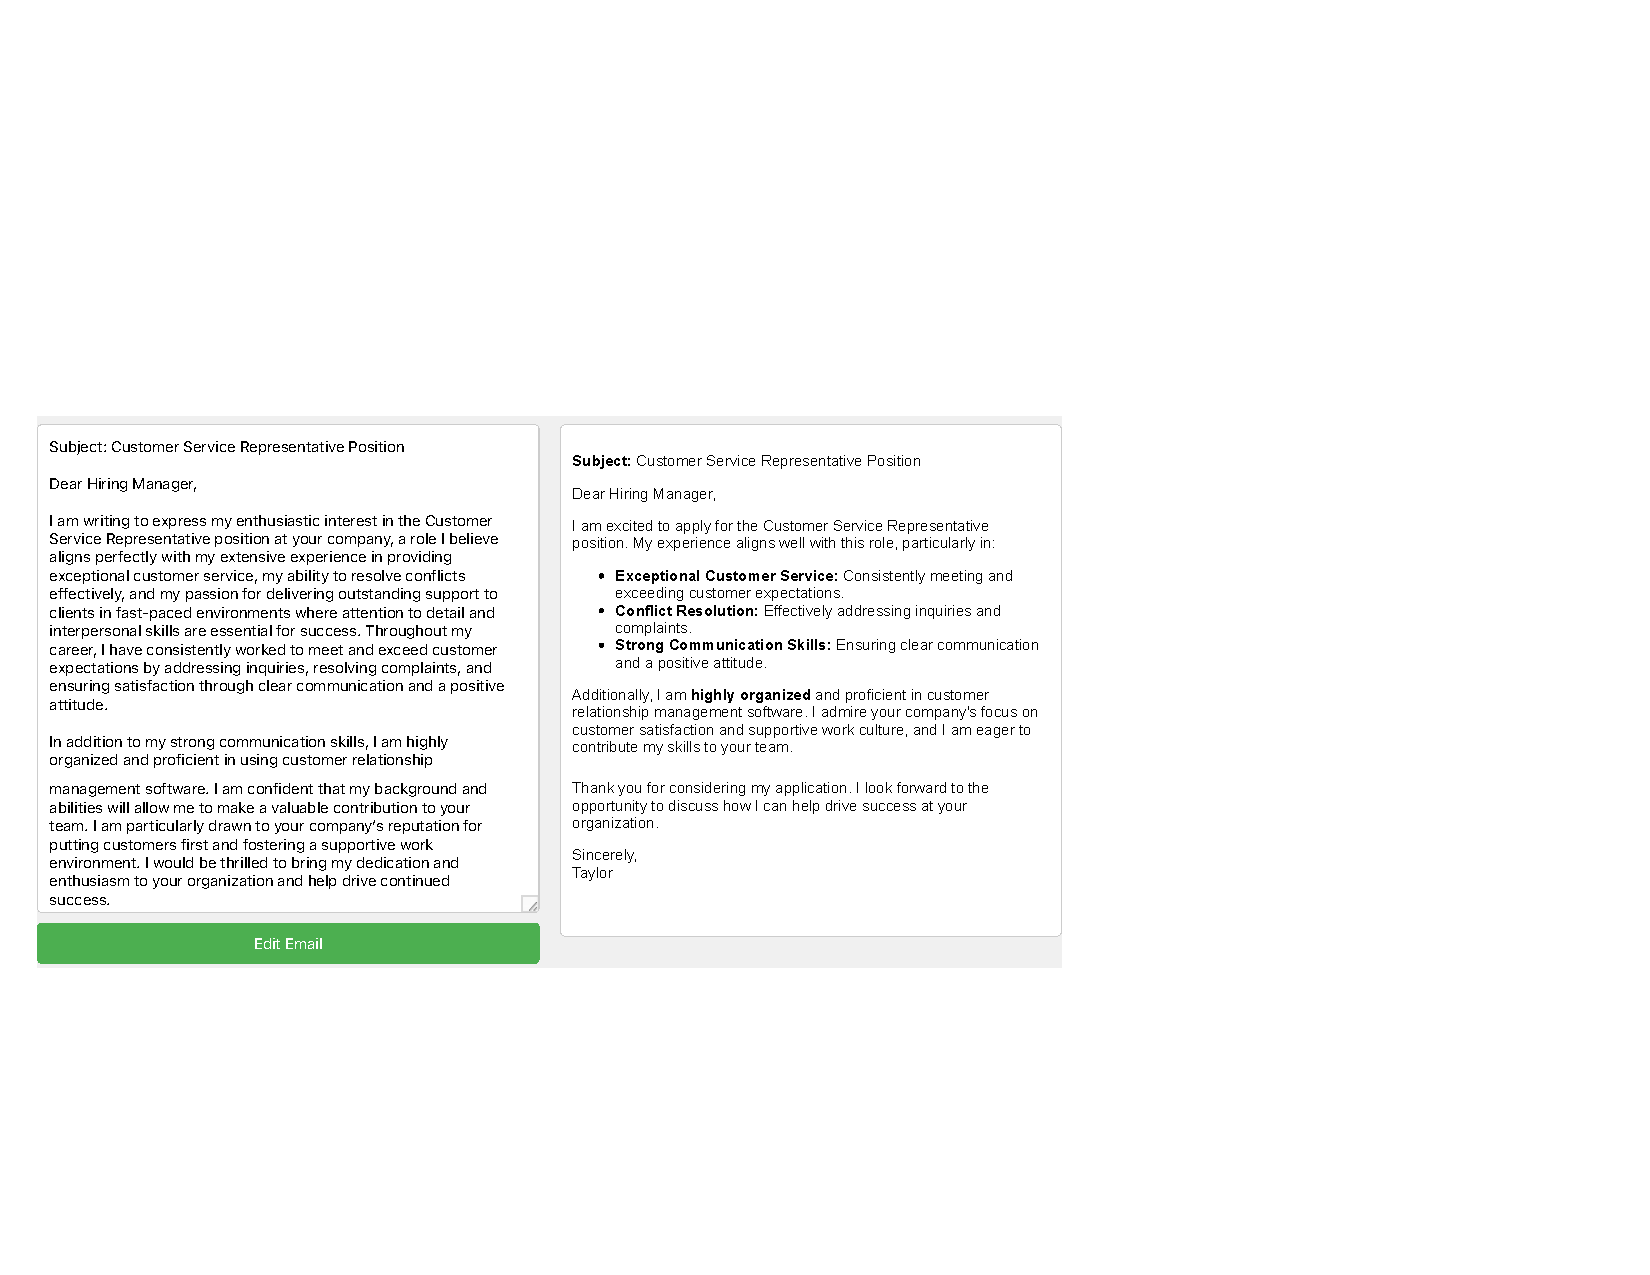
\includegraphics[width=.9\linewidth]{EmailRewriter.pdf}
    \caption{The AI writing tool we created for this investigation takes inputted text (left panel) and generates a version that incorporates recommended writing principles (right panel). Users could edit the text in the left-hand box, which was prepopulated with the text they were instructed to rewrite. They could then copy and paste the revised output from the right-hand box.}
    \label{fig:tool}
\end{figure*}

\begin{figure*}[]
    \centering
    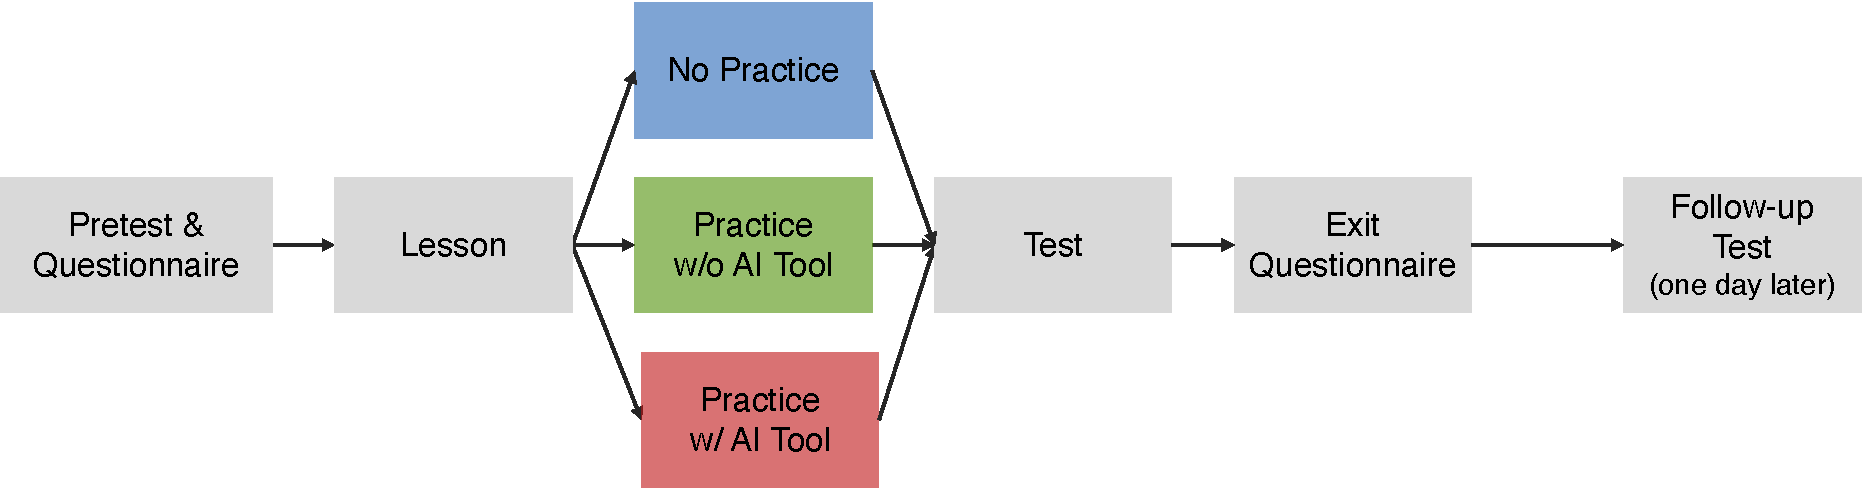
\includegraphics[width=.9\linewidth]{design_fig.pdf}
    \caption{Experimental design for Study 2. First, all participants completed a baseline questionnaire, a pretest (rewriting a poorly-written cover letter), and a lesson introducing five evidence-based principles of effective writing \cite{rogers2023}. Next, participants were randomly assigned to one of three conditions: practicing with an AI writing tool, practicing without an AI writing tool, or no practice. Then, all participants were tested on writing skill (rewriting a new cover letter without access to AI) and completed an exit questionnaire. Finally, to assess the persistence of skill improvement, participants were invited to complete a similar incentivized test of writing skill one day later.}
    \label{fig:design}
\end{figure*}

In Study 1, forecasters presented with this design were twice as likely to predict that practicing writing with the assistance of the AI tool would impair learning compared to practicing without the AI tool. 
In Study 2, however, participants who had practiced with the AI tool learned more (i.e., wrote better cover letters during the test phase) compared to either comparison group---an advantage that persisted in a one-day follow-up test. 
Finally, in Study 3, we explored the mechanism for these learning gains by introducing an example-only condition. 
Participants who had merely seen an AI-generated example (but did not have an opportunity to practice) improved in writing skill as much as participants who had practiced with an AI tool; benefits again persisted in a one-day follow-up test. 
Test-phase cover letters written by participants who had practiced with AI (Studies 2 and 3) or had seen an AI example (Study 3) were more likely to secure hypothetical job interviews compared to cover letters written by participants who had not practiced (Study 2) or had practiced without AI (Studies 2 and 3).

\section*{Study 1} 
\subsection*{Lay forecasters predicted that practicing with AI would hinder learning}

We showed \textit{N} = 150 participants screenshots of a random assignment study with three conditions.
  We asked them to rank-order these conditions according to how much they predicted future participants would learn in each. 
  Confirming our pre-registered hypothesis, nearly twice as many forecasters (64.7\%) ranked practicing alone above practicing writing with access to an AI tool as the converse (35.3\%, $\chi^2$ (1) = 12.9, \textit{p} < .001), see Figure \ref{fig:s1}. 
  Participants made this prediction regardless of self-reported experience with AI (\textit{OR} = 0.83, \textit{p} = .239) or any other measured demographic characteristic (\textit{p}s > .05).
  
\begin{figure}[]
    \centering
    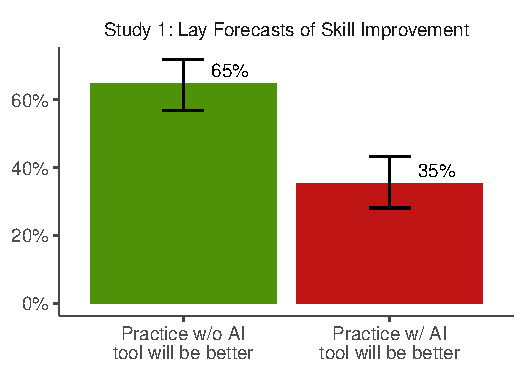
\includegraphics[width=1\linewidth]{ranking.pdf}
    \caption{Forecasters predicted that practicing without an AI tool would improve writing skill more than practicing with an AI tool. Error bars represent proportions $\pm$ 1 SE.}
    \label{fig:s1}
\end{figure}

In open-ended responses, forecasters who were pessimistic about the effect of the AI tool on learning speculated that it would crowd out effort (e.g., ``Practicing alone would force more recall and problem-solving skills, while AI essentially gives the answer for them.'', ``I think oftentimes using AI impedes the learning process because it's the `easy way.'''). Those with positive views, on the other hand, cited the possibility of AI providing insights or examples that would be otherwise unavailable (``As much as I hate AI, I do not believe you can improve in any manner if you do not have examples or ways of learning, and AI can provide this.'')



\section*{Study 2} 


Study 2 tested whether the predictions of Study 1 forecasters were
accurate. Specifically, \textit{N} = 2,238 participants completed a
baseline questionnaire and pretest (rewriting a poorly written cover
letter), followed by a lesson introducing five principles of effective
writing (i.e., Less is more, Make reading easy, Design for easy
navigation, Use enough formatting but no more, Make responding easy)
\cite{rogers2023}. 
Next, participants were randomly assigned to one of three practice conditions: (1) rewriting a new cover letter with an AI writing tool that revised text instantly based on these principles, (2) rewriting the new cover letter without the AI tool, or (3) a no practice control. 
At the end of the session, all
participants completed a test of writing skill (rewriting a yet another cover
letter without access to the AI writing tool) and an exit questionnaire.
One day later, all participants were invited to complete a similar
incentivized test of writing skill.


\subsection*{AI practice improved writing skill}

Consistent with other studies demonstrating the productivity benefits of
AI tools \cite{dellacqua2023, noy2023}, participants given access to the
AI writing tool produced cover letters during the practice phase that
were dramatically higher in quality than participants who were not
(\emph{d} = 1.01, \emph{p} \textless.001).

The learning advantage of having practiced with AI was evident in the
test phase: Consistent with our pre-registered hypothesis, participants
who had practiced with the AI tool produced higher-quality writing than did
participants who either had practiced without the AI tool (\emph{d} = .38,
\emph{p} \textless.001) or who had not practiced at all (\emph{d} = .47,
\emph{p} \textless.001). See Figure \ref{fig:s2_supplement}.
Likewise, cover letters written by participants who had practiced with AI were more likely to secure a hypothetical job interview than cover letters by participants who had practiced without AI (.54 vs. .50, \textit{p} = .002) or had not practiced at all (.54 vs. .47, \textit{p} < .001). See Figure \ref{fig:ratings1}. Notably, the effect of practicing with AI was not limited to stronger or weaker writers---participants across all skill levels benefited equally from practicing with AI. 

\begin{figure}[t]
    \centering
    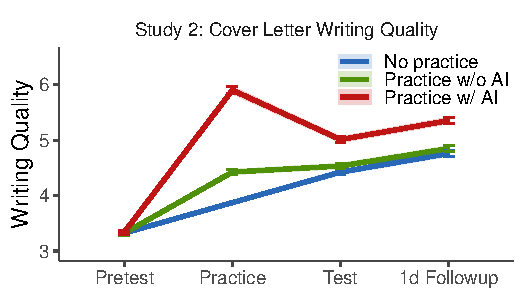
\includegraphics[width=1\linewidth]{mainfig.pdf}
    \caption{In both the main test and the follow-up, participants who had practiced with the AI tool outperformed those who practiced without it and those who did not practice at all.
    Error bars represent means $\pm$ 1 SE.
    Means shown are for the subsample of participants (\textit{n} = 1,294) who completed the one-day follow-up test. See Figure \ref{fig:s2_supplement} for the equivalent figure in the full sample, excluding the one-day follow-up phase (\textit{N} = 2,238).}
    \label{fig:difs}
\end{figure}

\begin{figure}[]
    \centering
    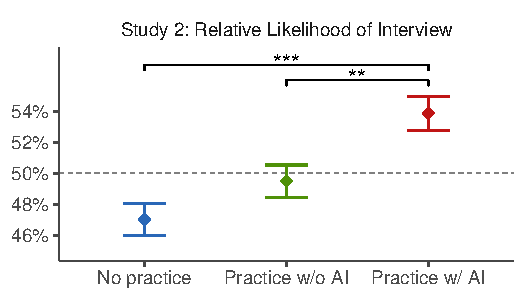
\includegraphics[width=1\linewidth]{ratings1.pdf}
    \caption{During the test phase, cover letters written by participants who had practiced with AI were more likely to lead to interview offers than those from other conditions. Points depict the average proportion of times each cover letter was preferred in pairwise comparisons with cover letters from the other two conditions. Error bars represent proportions $\pm$ 1 SE. The dashed line at 50\% represents no preference; values above this line indicate that cover letters were more likely to be preferred, while values below indicate they were less likely to be preferred.}
    \label{fig:ratings1}
\end{figure}

\subsection*{AI practice was less effortful}

The learning benefits of using an AI writing tool were evident
despite reduced effort during the practice phase. Compared to
participants who practiced alone, participants who practiced with the AI
tool spent 0.44 fewer minutes during the practice phase (3.73 vs.~4.17;
\emph{d} = -.12, \emph{p} = .025), logged roughly a quarter as many
keystrokes (26\% \emph{d} = -.44, \emph{p} \textless.001) and
self-reported expending less effort during practice (\emph{d} = -.31,
\emph{p} \textless.001).

Nevertheless, it would be inaccurate to label writers practicing with AI as entirely disengaged. 
  Copying, pasting, and submitting the AI tool's output could be accomplished almost instantly. 
  Yet, the majority of participants chose to interact with the task for over 3 minutes, and 95\% made at least one edit to the AI-generated output before final submission. See Figure \ref{fig:distance} in Supplementary Information for details.

Differential effort during practice raised the possibility that
participants who had practiced with the AI tool outperformed those who
had practiced on their own because they were less fatigued during the test
phase. However, participants who had practiced with AI did not spend more 
time as those who had practiced without AI (\emph{d} = .06, \emph{p} =
.235), but logged more keystrokes (\emph{d} = .12, \emph{p} = .026), and
self-reported expending less effort (\emph{d} = -.12, \emph{p} = .023)
during the test phase.

\subsection*{AI practice did not create the illusion of mastery}
Following the test phase, there were no differences by condition on
self-reported knowledge or motivation to improve. Despite improving more in objectively assessed writing skill, participants who had practiced with
AI reported having learned no more than those who had either
practiced alone or done no practice at all (\textit{p}s
\textgreater .05). Self-ratings of writing skill after the practice
phase were also indistinguishable between participants who practiced
with AI and those who practiced without the AI tool, or in the
no-practice control group (\textit{p}s \textgreater .05), but
participants who had practiced without AI rated their skill more highly
than those who did not practice (\emph{d} = .14 \emph{p} = .008).
Finally, compared to participants who did not practice, participants who had
practiced with AI were slightly less likely to request feedback after
the test phase (.65 vs.~.60, \textit{p} = .039), but just as likely as
participants who had practiced without AI (.64 vs.~.60, \textit{p} = .167).
See Section \ref{sec:future_learning2} in the Supplementary Information
for details.

\subsection*{The effects of practicing with AI persist}
To examine whether the treatment effects persisted over time, we re-contacted all
participants one day later. The majority of participants responded
(87\%), and attrition rates did not differ by condition (13\% to
14\% \(\chi^2\) = .68, \textit{p} .710). Confirming our pre-registered
hypothesis, participants who had practiced with the AI tool to practice the
previous day continued to outperform those who had practiced without the
tool (\emph{d} = .41, \emph{p} \textless.001) as well as those who had
not practiced at all (\emph{d} = .46, \emph{p} \textless.001).
Participants who had practiced without the AI tool performed no better
than those who did not practice (\emph{d} = .05, \emph{p} = .331). See Figure \ref{fig:difs} and Section \ref{sec:persists2} of Supplementary Information for details.

None of the findings above were moderated by individual difference
variables, including past experience with AI, age, gender, race,
education, motivation to learn, and baseline writing skill, BH-corrected
\textit{p}-values \textgreater .05. See Table \ref{tab:interactions2} in
the Supplementary Information for details.

\section*{Study 3}

\subsection*{Participants are willing to pay more for feedback from humans than for AI feedback}

\subsection*{Participants think editorial feedback is more effective, beyond social preferences}

\section*{Study 4}
\subsection*{Practicing with AI was more effective than looking for examples online and getting feedback from professional editors}

\subsection*{Practicing with AI is not less effortful than incorporating editorial feedback}

\subsection*{Practicing with AI does not create more of an illusion of knowledge than editorial feedback}


\section*{Study 5} 

To gain insight into what might be driving the benefit of practicing with AI, in Study 3 (\emph{N} = 2,003), we preregistered a replication and extension in which we replaced the no-practice condition of Study 2 with an example-only condition.
In this condition, participants were shown an AI-generated writing example that they could not edit. 
To the extent that the benefit of practicing with AI was driven by exposure to examples, the example-only condition should improve performance in the test phase as much as the practice with AI condition.

\subsection*{Seeing an AI example was as effective as practicing with
AI}\label{seeing-an-ai-example-was-as-effective-as-practicing-with-ai}

As in Study 2, participants given access to the AI writing tool dramatically outperformed participants who did not get access to it, both while using it during the practice phase (\emph{d} = 1.22, \emph{p} \textless.001), and during the no-AI test phase (\emph{d} = .34, \emph{p}  \textless{} .001). Their test-phase cover letters were also relatively more likely to secure them hypothetical job interviews (.51 vs. .47, \textit{p} = .008).

Participants who had merely seen an AI-generated example also improved more in writing skill than those who had practiced without AI (\emph{d} = .37, \emph{p} = \textless{} .001), and produced letters that were relatively more likely to secure them interviews (.52 vs. .47, \textit{p} = .007). Notably, they improved as much as participants who had practiced with the AI tool (and could edit its output, \emph{d} = .03, \emph{p} = .883), and were offered hypothetical interviews at similar rates as them (.51 vs. .52, \textit{p} = .561). See Figures \ref{fig:s3sup} and \ref{fig:ratings2}. As in Study 2, gains from practicing with AI and seeing AI examples were comparable across all levels of baseline writing skill.

\begin{figure}[t]
    \centering
    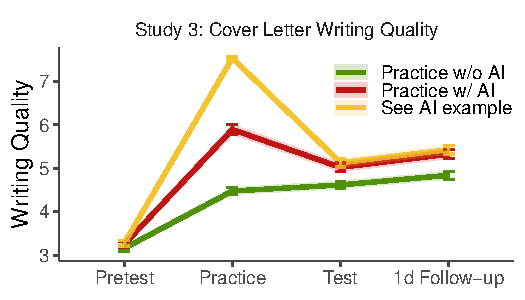
\includegraphics[width=\linewidth]{average_test_rewritten_lines_raw.pdf}
    \caption{
    In both the main test and the follow-up, participants who simply saw an AI-generated example improved just as much as those who practiced with AI and more than those who practiced without AI.
    Error bars represent means $\pm$ 1 SE.
    Means shown are for the subsample of participants  (\textit{n} = 608) who completed the one-day follow-up test.
    See Figure \ref{fig:s3sup} for the equivalent figure in the full sample, excluding the one-day follow-up phase (\textit{N} = 2,003).}
    \label{fig:s3}
\end{figure}

\begin{figure}[]
    \centering
    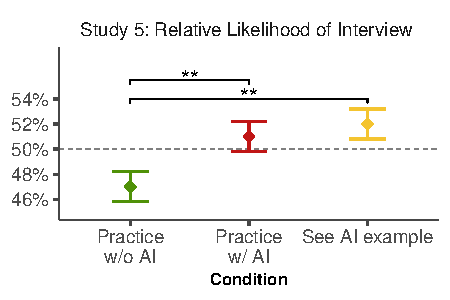
\includegraphics[width=1\linewidth]{ratings2.pdf}
    \caption{During the test phase, cover letters written by participants who had seen an AI-generated example were about equally likely to lead to interview offers when compared to those assigned to practice with AI. Cover letters from both AI conditions outperformed those written by participants who were assigned to practice without AI. Points depict the average proportion of times each cover letter was preferred in pairwise comparisons with cover letters from the other two conditions. Error bars represent proportions $\pm$ 1 SE. The dashed line at 50\% represents no preference; values above this line indicate that cover letters were more likely to be preferred, while values below indicate they were less likely to be preferred.}
    \label{fig:ratings2}
\end{figure}




\subsection*{Seeing an AI example was even less effortful than practicing
with
AI}\label{seeing-an-ai-example-was-even-less-effortful-than-practicing-with-ai}

During the practice phase, participants who saw the AI example spent 2.32 fewer minutes than participants
practicing with AI (\emph{d} = 0.99, \emph{p} \textless{}
.001) and 2.96 fewer minutes than participants practicing without AI (\emph{d} =
1.13 \emph{p} = \textless{} .001), and reported expending less effort than those practicing with an AI tool
(\emph{d} = 0.19, \emph{p} = .003) and those practicing without AI (\emph{d} = 0.32, \emph{p}
\textless{} .001).  As in Study 2, participants who practiced with AI logged 2.83 times fewer keystrokes than did participants who practiced without AI. As expected, participants exposed to the AI example logged 0 keystrokes.

During the test phase, participants who had seen the AI example worked for an additional 56 seconds more than participants who had practiced without AI (\emph{d} = 0.22, \emph{p} \textless{} .001). They also logged 30\% more keystrokes than participants who had practiced with AI (\textit{d} = 1.86 \textit{p} <.001) and 60\% more than those who practiced without AI (\textit{d} = 2.39, \textit{p} < .001). Across conditions, all participants self-reported similar levels of subjective effort (\textit{d}s < .08, \textit{p}s > .05).

\subsection*{Seeing an AI example did not create the illusion of mastery}

As in Study 2, despite learning more, participants who had practiced with AI or had merely seen an AI-generated example reported learning similar amounts to those who practiced without AI (\textit{p}s > .05) and rated their writing skill after practice at comparable levels (\textit{p}s > .05). Moreover, all participants requested feedback at similar rates (proportions ranged from 63\% to 67\%). See Section \ref{sec:future_learning3} in the Supplementary Information for details.


\subsection*{The effects of seeing an AI example
persist}\label{the-effects-of-seeing-an-ai-example-persist}

When we recontacted a subsample of (\textit{n} = 800) participants one day later, 
  the majority responded (\textit{n} = 633, 80\%); the attrition rates ranged from 17\% to 24\% and did not differ by condition ($\chi^2$ (2) = 4.56, \textit{p} = .102).
  The effect remained robust after 24 hours. Participants who had practiced with the AI-tool (\emph{d} = .29, \emph{p} = .006) and participants who had simply seen an AI example (\emph{d} = .32, \emph{p} = .003), both continued to outperform those who had practiced without the tool. Participants who had merely seen an AI example performed as well as those who had practiced with AI (\emph{d} = .02, \emph{p} = .830). See Figure \ref{fig:s3} and Section \ref{sec:persist3} of Supplementary Information for details.

As in Study 2, the above findings were not moderated by individual differences. See Table \ref{tab:interactions3} in the
Supplementary Information for details.




\section*{Discussion} 
% Contrary to the expectations of lay forecasters (Study 1), participants who relied on an AI tool to write cover letters improved in writing skill compared to participants who practiced alone (Study 2).

Add a discussion paragraph on effort. People think that more effort causes learning. But no, we found that AI users never worked harder and always learned more. AI can remove the unnecesary effort, and thus help you be more efficient with the effort you put in. 

Contrary to the expectations of lay forecasters (Study 1), participants who practiced writing cover letters with an AI tool learned more than those who practiced on their own (Studies 2 and 3). Specifically, participants who had practiced with AI wrote (without AI assistance) cover letters that were rated higher in writing quality and were more likely to secure a hypothetical interview---both immediately after practice and one day later.
Learning gains were not the result of greater effort; in fact, participants who'd practiced with AI expended less effort during practice than those who'd practiced alone. Instead, these gains can be explained by exposure to a high-quality, just-in-time personalized example: participants who merely viewed an AI-generated example cover letter (without editing it) improved their writing skill as much as those given the option to practice editing the cover letter (Study 3).

While not obvious to forecasters, teachers \cite{lin2024a}, and the general population \cite{hawkins2024between}, the benefits of seeing AI-generated examples are consistent with prior research on how people learn. 
 In addition to the literature on worked examples mentioned earlier, research has shown that humans are especially adept at observing, imitating, and learning from others \cite{bandura1971, meltzoff2005imitation, lyons2007hidden}. 
  Our findings also align with the expert performance literature: the most successful learners engage in deliberate practice, which (in addition to concentration, feedback, and repetition) depends upon detailed mental representations of excellent performance \cite{anders2008deliberate}.   

\subsection*{Future Directions}
Three promising directions for future research are worth highlighting.
First, it remains to be seen whether learning from AI examples occurs in domains other than writing, currently the modal use case for AI tools in the workplace \cite{bick2024rapid}. Writing may be particularly suited to learning by example because at a glance, a single AI-generated example visually communicates the elements of effective professional writing (e.g., short sentences and boldface formatting). 
    In other domains, merely observing a solution may be less informative. For instance, the final answer to a math or computer programming problem does not instantly reveal the procedure that produced it. Studies of AI tutors in these domains have, perhaps not surprisingly, found null or negative effects \cite{bastani2024, nie2024gpt}.    

   

    
Second, additional research is needed to explore moderators of learning from AI tools. 
    Certain strategies for interacting with AI may bolster their effectiveness.
    For example, experimental research suggests that learners benefit more from AI explanations for math problems if they first try to solve them on their own \cite{kumar2023}. 
    Similarly, correlational evidence that asking AI for explanations as opposed to answers is associated with more learning in mathematics \cite{bastani2024} and computer programming \cite{lehmann2024ai}.
    On the other hand, other factors could minimize learning benefits.
    In our experimental paradigm, participants practiced for as long as they wanted, with the foreknowledge that their skills would subsequently be tested (and rewarded monetarily) without access to AI. 
    During practice, therefore, participants were incentivized to prioritize gains in acquired skill over performance in the moment. 
    In real-world settings, there is often time pressure and competing incentives around performance and learning, which we speculate would reduce the learning gains associated with practicing with AI.

Third, in our experimental paradigm, participants who interacted with the AI tool did so only once. 
  It is common, however, to use AI tools repeatedly. 
  When do repeated interactions lead to diminishing or even negative returns, and in what scenarios might skill development continue over time?  Consider, for instance, the game of Go. The introduction of superhuman AI has been associated with an increase in the novelty and quality of decisions made by human Go players over time, with elite players reporting that they have been inspired by AI solutions they'd never seen before \cite{shin2023}.     
  Future research, ideally in field settings, is needed to establish the long-term benefits and costs of relying on AI tools.


\subsection*{Conclusion}
Our findings should temper widespread concern that AI tools invariably boost momentary productivity at the expense of long-term skill development.  
  Although it reduced the effort users invested in practicing, the AI writing tool nevertheless accelerated skill development.
  It accomplished this by providing high-quality, just-in-time, personalized examples of excellent writing.
  The underappreciated efficacy of timely and tailored examples has practical implications for the design of AI tools. 
  Many AI tools designed to support learning are explicitly programmed not to ``give away'' answers. 
  It may be that in addition to hints, leading questions, and explanations, learners benefit from demonstrations of the principles they are attempting to master.
  
  Decades before the advent of generative AI, the legendary UCLA basketball coach John Wooden declared that the four laws of learning are explanation, demonstration, imitation, and repetition \cite{whut2010}. 
  Few learners have access to the best human teachers, coaches, and mentors, but generative AI now makes it possible to learn from personalized, just-in-time demonstrations tailored to any domain. 
  In doing so, AI has the potential not only to boost productivity but also to democratize opportunities to build human capital at scale.

\section*{Methods}
\subsection*{Ethical Considerations}
The study was assessed by the University of Pennsylvania's IRB, and was approved before implementation (Protocol 853653). All participants completed informed consent.

\subsection*{Pre-registration}
All our studies were pre-registered. See pre-registrations for Study 1 at https://aspredicted.org/x9mm-7qwp.pdf. 

Study 2 was run twice because of a technical issue that caused imbalanced missing data issue the first time it was run. 
  The findings in this sample were consistent with the ones reported here. 
  Pre-registration is available at https://aspredicted.org/4sw4-mpny.pdf. 
  The version of Study 2 presented above was pre-registered https://aspredicted.org/xyyn-gmzc.pdf. 

Pre-registration for Study 3 is available at https://aspredicted.org/3mty-fcfy.pdf. 
  The one-day follow-up for Study 3 was collected in three batches. 
  We pre-registered batch 2 https://aspredicted.org/5jcx-bhg9.pdf, but report pooled results in the main text. 
  Details on the separate batches are available in Supplementary Information Section \ref{sec:persist3}.

\subsection*{Participants}
We sampled participants from Prolific from all our studies. We excluded all Prolific users who participated in one of the earlier studies from participation in subsequent studies. 

Participants in Study 1 (\textit{N} = 150) were predominantly female (n = 93, 62\%), and ranged in age from 21 to 81 (M = 38.4, SD = 12.2). They were predominantly white (75\%). A small proportion were students (13\%), and most were employed (62\%)

In Study 2, the sample was more evenly split between men (46\%) and women (52\%), and ranged in age from 18 to 82 (M = 36.0, SD = 12.5). Over half of the sample (58\%) was white, with the rest being comprised by Black (33\%), latino (6\%), and asian (5\%). 77\% had college degrees. Most participants (93\%) were at least somewhat motivated to improve their writing, and had varying levels of experience with AI writing assistants (36\% had tried them, but hardly ever used them, 47\% used them at least a few times per week, and 17\% had never used AI assistants before).

Study 3 had similar proportions of men (46\%) and women (53\%), and participants ranged in age from 18 to 95 (M = 37.9, SD = 12.6). Over half of the sample (64\%) was white, with the rest being comprised of Black (24\%), Latino (8\%), and Asian (6\%) participants. Most participants (74\%) had college degrees. Most participants (91\%) were at least somewhat motivated to improve their writing, and had varying levels of experience with AI writing assistants (40\% had tried them, but hardly ever used them, 42\% used them at least a few times per week, and 18\% had never used AI assistants before).

\subsection*{Procedure}
Participants first saw an introductory screen about what they were about to do. 
  They then completed a brief questionnaire where they reported their demographics, their experience with AI writing tools, their motivation to improve their writing, and their perceived writing skill. 
  They then completed a 2-minute pre-test in which they saw a poorly worded cover letter and were asked to improve it. 
  After this, all participants completed a lesson about the five principles of effective writing. 
  They were then randomized to the practice condition, or skipped ahead if assigned to the no-practice control. 
  During the practice phase, participants rewrote a different cover letter, or (in the see example condition) generated an AI rewritten version of that letter. 
  This example was not explicitly labeled as AI-generated.
  Then, participants saw the text they submitted (or the AI-generated example), and below it, AI-generated feedback highlighting one way in which this letter could be improved. See more information about the feedback procedure in Supplementary Information section \ref{sec:feedback}.
  Immediately after seeing this feedback screen, all participants then completed two questions, reporting how much they had learned and how hard they had worked on the task so far. 
  They then edited a new cover letter in an incentivized, 7-minute test without the help of any AI tools. 
  To minimize the possibility of cheating, we used custom JavaScript to restrict copy-pasting functionality. 
  Finally, participants were invited to see optional feedback and were asked if they had used any outside resources during the test. 
  
A small percentage of participants (2.88\%) admitted to cheating. 
  As per our pre-registration, these participants are included in our analyses, but see Tables \ref{tab:s2_test} and \ref{tab:s3_test} in Supplementary Information to see results excluding them, which are consistent with our main interpretation.

\subsection*{Measurement}
As per our pre-registration, we used OpenAI's GPT-4o to rate text samples for writing quality. 
    To do this, we independently rated each cover letter and each writing principle. 
    Research has demonstrated that large language models can provide ratings of writing quality that align closely with human judgments, offering reliability and consistency across various evaluation contexts \cite{rathje2024, hackl2023}.
    See our prompts in Table \ref{tab:prompts}. 
    We then took the unweighted average of these 5 scores as our main dependent variable. 
    See disaggregated analyses by each writing principle and additional outcomes on Table \ref{tab:s2_test} and \ref{tab:s3_test}.

To validate these ratings, the first author and a trained research assistant took a sample of \textit{n} = 30 cover letters from Study 2, and rated them on the 5 principles. The average of these two ratings correlated more highly with the computer ratings (\textit{r} = .83, \textit{p} < .001), than the average interrater reliability (\textit{r} = .69, \textit{p} < .001).

To address concerns that particular LLMs might be biased in favor of their own output, we also used Claude to rate the cover letters. We find that GPT ratings correlate strongly with Claude ratings (\textit{r} = .71, \textit{p} < .001), and that the effects are not attenuated by using different models (See Tables \ref{tab:s2_test} and \ref{tab:s3_test}), suggesting that our effects are not explainable by same-model bias.

\subsection*{Statistical analysis}
As per our pre-registrations, we fit ANCOVA models predicting outcomes from condition indicators, controlling for pretest score and baseline characteristics (age, gender, race/ethnicity, primary language, education level, motivation to improve writing skills, self-rated writing skill, experience with AI writing assistants, and baseline writing effectiveness). We used logistic regression to predict whether participants chose to see optional feedback for their test from condition, controlling for pretest score and baseline characteristics. 
Our analyses of the hypothetical hiring situation use beta regression, because the relative likelihood of a cover letter being preferred is bounded between 0 and 1.
When correcting for multiple comparisons in exploratory moderation analyses, we use the Benjamini-Hochberg correction \cite{benjamini1995controlling}. 


END


\chapter{Khan}

Can generative AI provide motivational support at scale? 
While psychological interventions have proven to be effective in controlled settings, their scalability in natural contexts remains understudied. 
This year-long field investigation shows that AI-delivered interventions benefit learners in an ecologically valid setting.
Relative to the week before completing the intervention, students increased their time on task by 53\% after Situation Modification and 75\% after Emotional Reframing. 
Students also worked on more challenging items following exposure to the interventions.
Effects on accuracy were less robust: average accuracy did not improve, but under Emotional Reframing higher-skill students showed modest gains.
% Although our design was observational rather than randomized, analyses suggest minimal selection biases. Users exhibited similar patterns of activity before engaging with the interventions, with the exception that they attempted more challenging items and spent more total time on task during this period for the emotional reframing and situation modification prompts, respectively. Our analysis additionally controls for all unobserved user characteristics, general time trends, and time-varying user skill. 
Exploratory text analyses reveal that AI-facilitated interactions are associated with reduced negative affect.
These findings suggest that scalable emotion regulation interventions can significantly enhance engagement in digital learning environments, highlighting the potential for AI-supported emotional scaffolding to address barriers to educational persistence and achievement.


Motivation is a central driver of behavior in various domains, including consumer decision-making, workplace performance, health, and education. 
People often know what they should do---whether it’s sticking to a fitness plan, managing personal finances, or completing an online course---yet struggle to persist when faced with frustration, effort, or competing demands. 
A core challenge in behavior change is not just delivering information but sustaining motivation over time.

% There is a literature in affective computing that has traditionally focused on the emotional and motivational challenges of learning, but hasn't been able to do this at scale and with interactivity. 
% They have been primarily on controlled lab settings, e.g, in labs to record facial expressions and detect affect from that.

Traditionally, human mentors, managers, or coaches provide this motivational support, recognizing when individuals are struggling and intervening in real-time (Lepper et al., 1993). 
However, as interactions shift to digital environments, this personalized, adaptive motivational support is often missing. 
The consequences are well-documented: employees disengage from workplace training, consumers abandon long-term financial plans, and learners drop out of online courses (Reich \& Ruipérez-Valiente, 2019; Milkman et al., 2021). 
Without timely intervention, engagement and persistence decline, limiting the effectiveness of digital interventions.

\subsection*{The Process Model of Emotion Regulation}
Psychological research offers a promising framework for addressing these motivational failures. 
The process model of emotion regulation (Gross, 1998) describes how individuals respond to challenges that trigger frustration, anxiety, or disengagement from a task. 
The model identifies two key strategies that proactively shape emotional responses:

\subsubsection*{Situation modification} 
Structuring the environment to reduce the need for willpower. 
In a workplace setting, this might involve removing distractions to enhance productivity. 
In consumer finance, it could mean automating savings to prevent impulsive spending.

\subsubsection*{Emotional reframing} Interpreting negative emotions (e.g., frustration) as signals of progress rather than failure. 
For instance, framing difficulty as a necessary step in skill development can increase persistence in learning, just as reframing discomfort in exercise can encourage continued effort.

Behavioral interventions based on these strategies have successfully improved consumer persistence, workplace performance, and learning outcomes (Yeager et al., 2016; Mrazek et al., 2018). 
However, scaling these interventions remains a challenge—particularly in digital settings where human coaches are unavailable.

\subsection*{AI as a Scalable Motivational Coach}
Advances in AI-powered conversational agents offer a potential solution, providing real-time, scalable motivational support at a fraction of the cost of human mentors. 
There are three reasons why generative AI may effectively support motivation and learning.

First, people generally perceive text written by AI assistants as empathetic, sometimes more so than text written by humans. 
Perceived empathy: Research suggests that AI can sometimes be viewed as more supportive than humans, particularly in digital interactions where social judgment is minimized (Hoegen et al., 2019).

Personalization and engagement: Unlike static behavioral interventions, modern generative AI can adapt advice in real-time, tailoring motivational support to individual users (Bickmore et al., 2005).

Scalability: AI can provide instant, on-demand motivation across millions of users, making it far more cost-effective than human coaches.

However, AI-driven motivation may also fail for two reasons:

Human connection may be essential: Theories of social learning suggest that motivation is facilitated by authentic human connection. 
Studies on early childhood language acquisition, for example, show that children cannot learn from passive digital exposure alone (Kuhl, 2007). 
If motivation operates similarly, AI-based interventions may be insufficient.

AI can make mistakes: Prior research has shown that AI-generated advice—particularly in sensitive areas like mental health—can be misleading or counterproductive (Stefanos et al., 2023). 
Poorly timed or irrelevant motivational interventions could frustrate users rather than support them.

\begin{figure*}
    \centering
    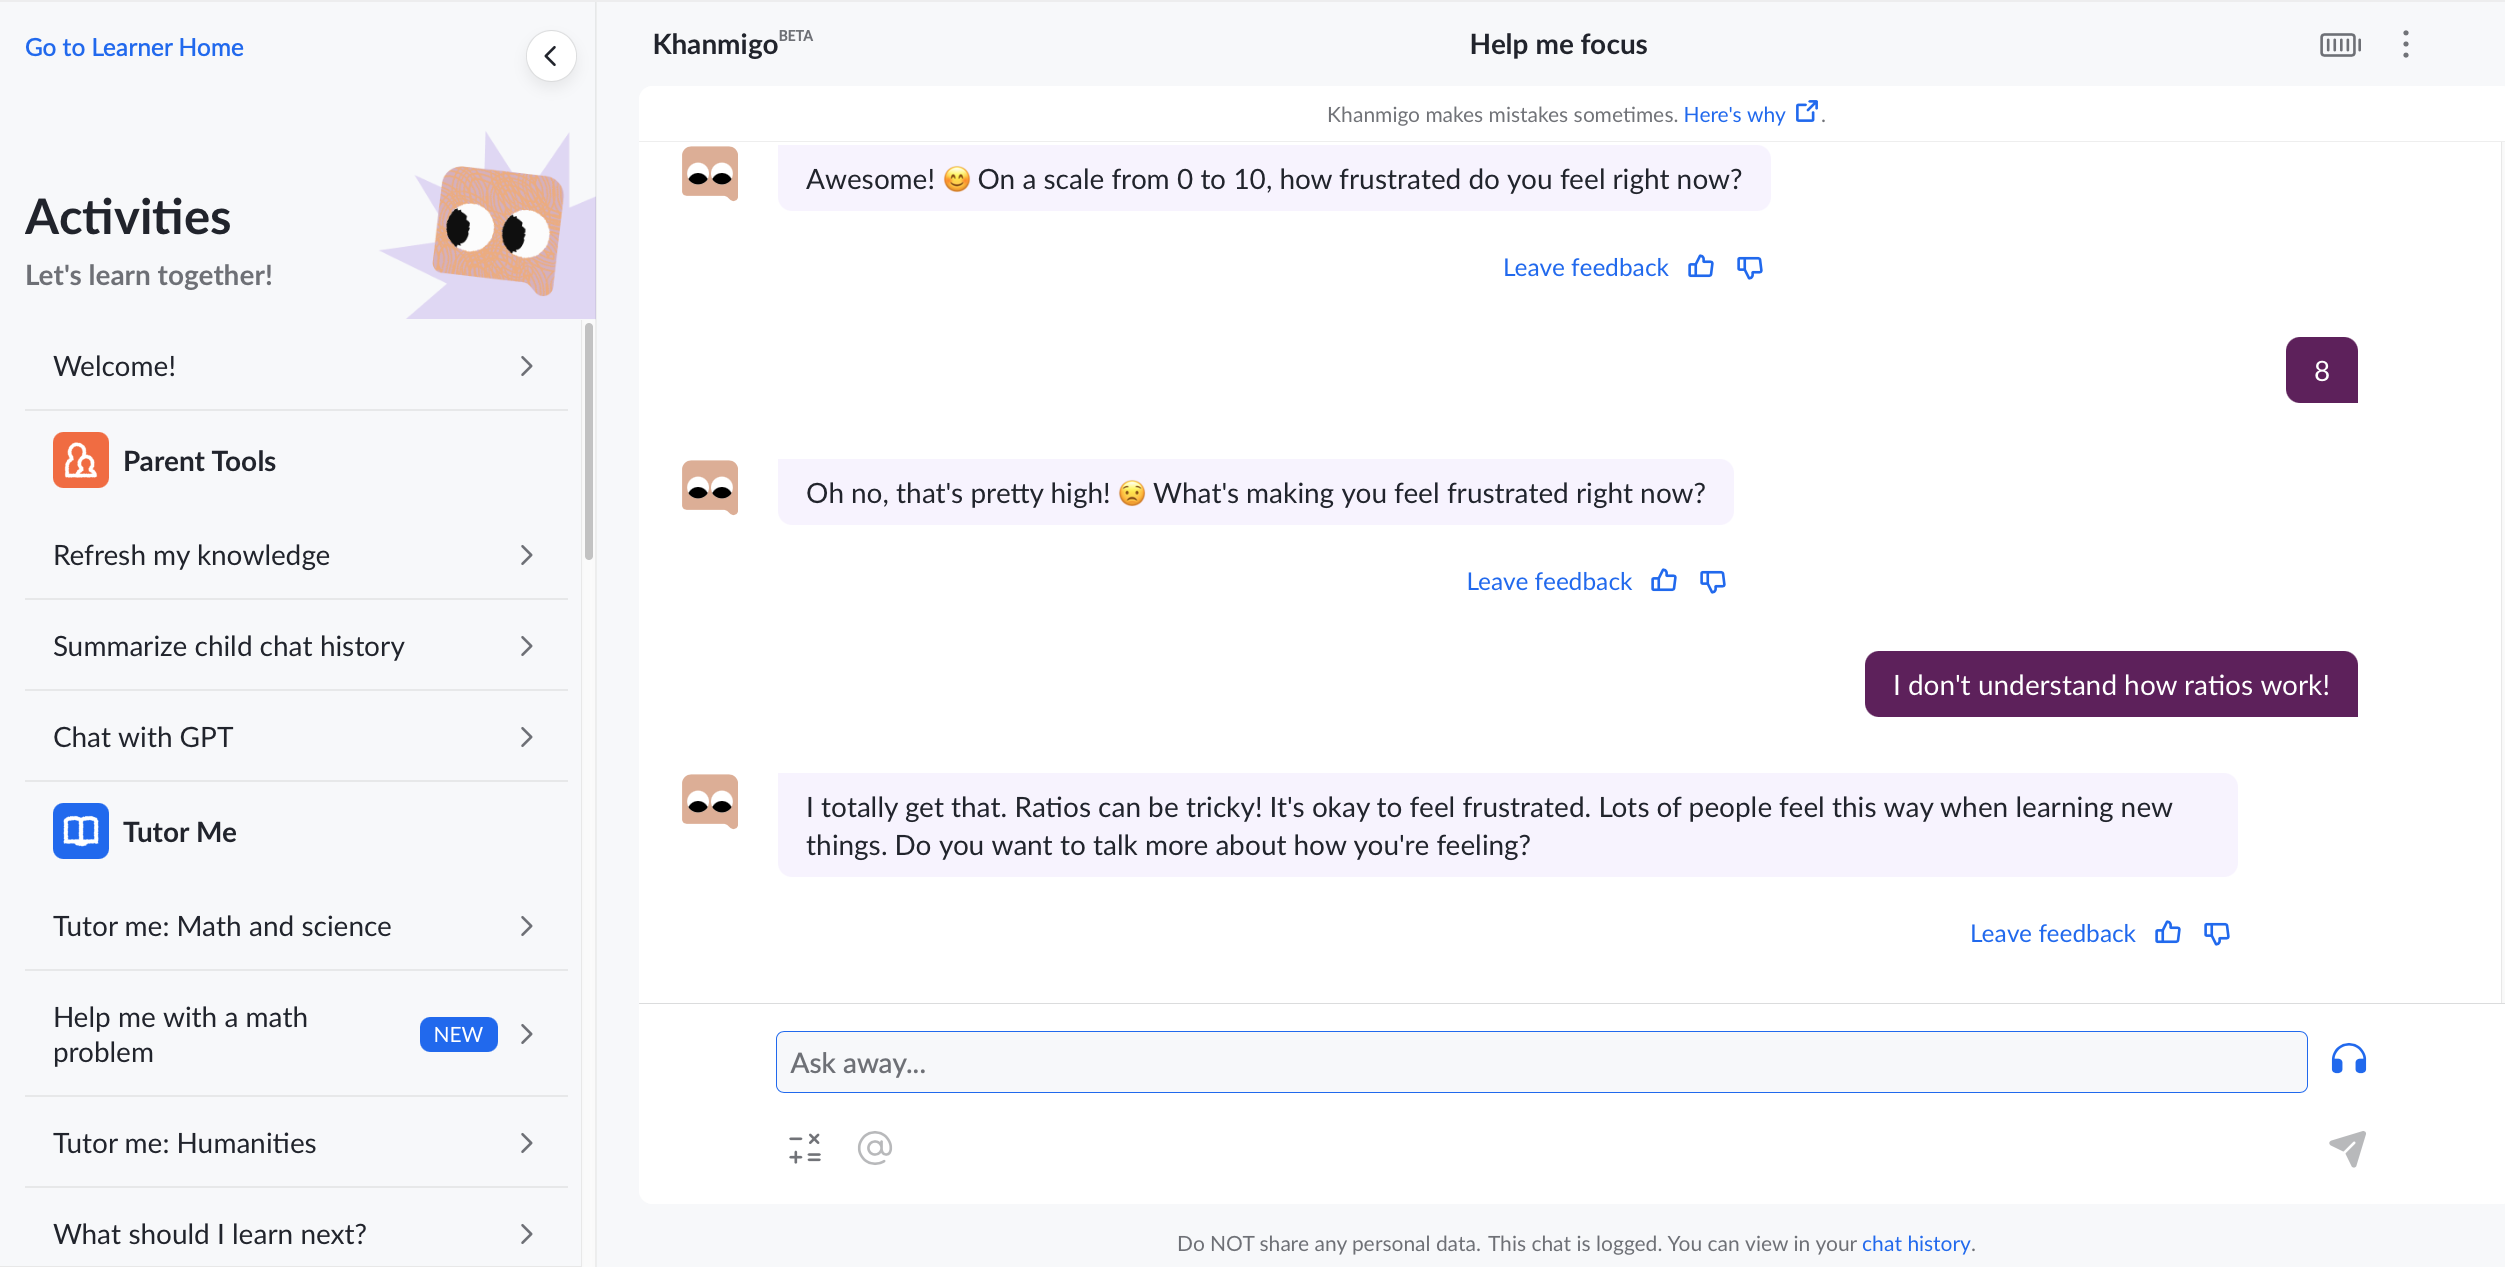
\includegraphics[width=0.95\linewidth]{figure/interface.png}
    \caption{The interface that the users saw when they decided to engage with the bot.}
    \label{fig:interface}
\end{figure*}

\begin{figure}
    \centering
    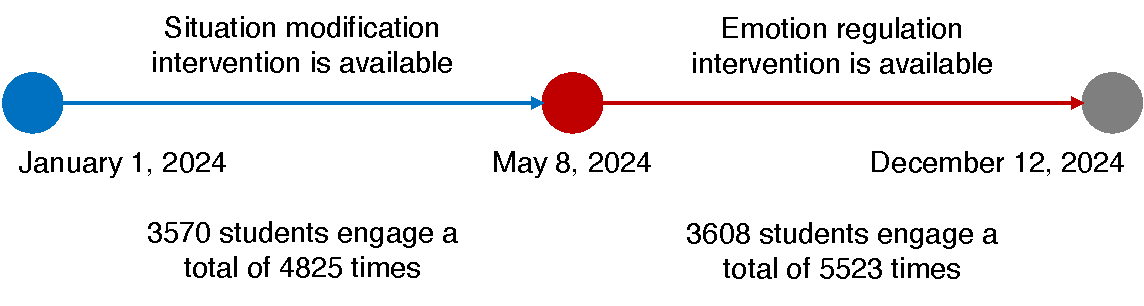
\includegraphics[width=0.95\linewidth]{figure/sample.pdf}
    \caption{Data collection times and sample sizes.}
    \label{fig:sample}
\end{figure}


\subsection*{Current Investigation}
This study presents the first large-scale, year-long observational analysis of AI-powered motivational coaching in a digital performance setting. 
Using behavioral data from Khan Academy, we evaluate two AI-driven motivational strategies:

\subsubsection*{Situation modification} Encouraging users to structure their environment and habits in ways that reduce reliance on willpower.
\subsubsection*{Emotional reframing} Helping users reinterpret frustration as an expected and productive part of progress.
 
Since AI usage was self-selected, this study does not constitute a traditional experiment. 
Instead, we employ a fixed-effects methodology to account for timing and user heterogeneity, controlling for time-varying confounds through Bayesian item response theory (IRT) estimates of skill and motivation. 
This approach allows us to isolate the impact of AI-driven motivational interventions from broader shifts in user performance over time.

By evaluating AI-driven motivation at scale, this study makes three key contributions:

AI in behavioral interventions: Can AI effectively sustain engagement and persistence across digital performance environments?
The role of human interaction in motivation: Does AI-based motivation substitute for or complement human-delivered support?
Scalability of motivation science: How can emotion regulation strategies be embedded into AI systems to drive persistence in learning, work, and decision-making?

Beyond education, these findings have broad implications for AI-driven behavioral interventions in domains such as employee training, consumer engagement, and digital health. 
As AI systems increasingly mediate human decision-making, understanding when and how AI can sustain motivation is a critical question for marketing, management, and behavioral science.

\section*{Results} 

\subsection*{When do users decide to engage with the prompts}
Because students could choose when to engage with the interventions, our first step was to examine the timing of that choice.
If students tended to use a prompt when they were already disengaged or performing poorly, any apparent post-intervention improvement could simply reflect regression to the mean.
Our data suggest this was not the case. 

We compared user activity in the week before prompt use to a one-month baseline and found no evidence of systematic dips in engagement or performance preceding the intervention (Figure~\ref{fig:when_engage}). 
In fact, students were more likely to use the situation modification prompt during periods of above-average activity, and to use the emotional reframing prompt when they had recently been attempting more difficult items.


\begin{figure}
    \centering
    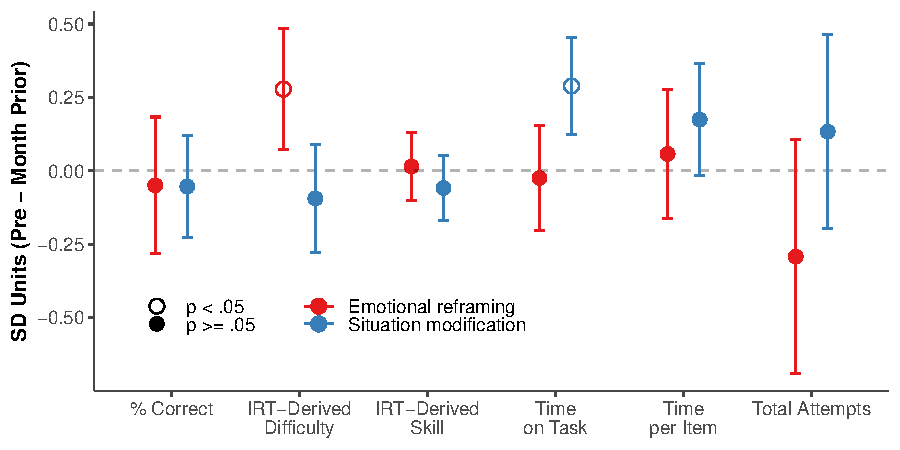
\includegraphics[width=\linewidth]{figure/when_engage.pdf}
    \caption{Users chose to engage with the prompts at times that were, for the most part, comparable to baseline. However, they were more likely to click on (1) the Emotional Reframing bot when they had been working on harder problems, and (2) the Situation Modification prompt when they had accumulated more time on task than usual. Baseline = One month before the pre-intervention period.}
    \label{fig:when_engage}
\end{figure}

\subsection*{Chatbot use is related to increases in motivation but not performance}

As preregistered, students spent significantly more time working during the following week. 
Specifically, they worked **53\%** longer after Situation Modification (\(\beta=0.426,\ p<0.001\)) and **75\%** longer after Emotional Reframing (\(\beta=0.558,\ p<0.001\)).

This increased engagement did not translate into higher performance, contrary to our pre-registered hypothesis. 
In the week following either prompt, students did not show a significant improvement in accuracy (Situation Modification: \(\beta=0.425,\ p>0.05\); Emotional Reframing: \(\beta=0.586,\ p>0.05\)).

Exploratory pre-registered analyses suggest that after engaging with the chatbot, users attempted more difficult items. 
This suggests that chatbot users may challenge themselves more, even if this does not immediately translate to higher accuracy. See Table \ref{tab:main_reg} and Figure \ref{fig:main}.

Our exploratory analyses provide additional context for these findings. 
The positive post-intervention coefficients for difficulty (\(\beta=0.129,\ p<0.001\) for Situation Modification; \(\beta=0.119,\ p<0.001\) for Emotional Reframing) indicate that users attempted more challenging items after interacting with the chatbot. 
This increased willingness to tackle difficult problems aligns with the observed increase in engagement duration, suggesting that chatbot use may enhance user confidence or motivation.

As expected, user skill was strongly associated with higher accuracy ($\beta$ = 61.608, \textit{p} < 0.001 for situation modification; $\beta$ = 68.997, \textit{p} < 0.001 for emotional reframing), longer engagement durations, and willingness to attempt more difficult items. 
Similarly, item difficulty was negatively associated with accuracy and engagement duration.

\begin{figure}
    \centering
    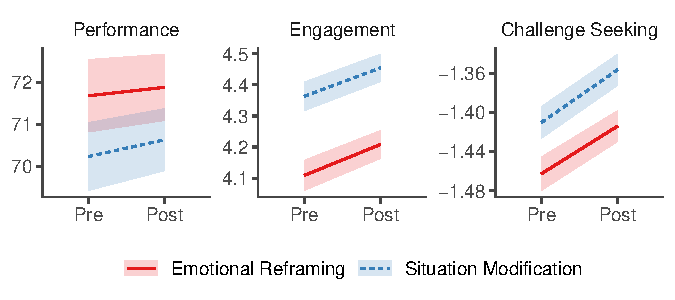
\includegraphics[width=\linewidth]{figure/main.pdf}
    \caption{After students engaged with the situation modification and emotion regulation prompts, they saw increases in their motivation (operationalized as total time on task), and the difficulty of the items they attempted. 
    There were no detectable effects on skill as measured by the proportion of correct responses. 
    Results adjust for general time trends, all time-invariant student characteristics, item difficulty, and student's time-varying skill levels.}
    \label{fig:main}
\end{figure}

\begin{landscape}
\begin{table*}[!htbp] \centering    \caption{Regression Results}    \label{tab:main_reg} \resizebox{\textwidth}{!}{% key: fit to the (rotated) page height
\begin{tabular}{@{\extracolsep{5pt}}lcccccc}  \\[-1.8ex]\hline \\[-1.8ex]  \\[-1.8ex] & \multicolumn{2}{c}{Engagement: Log(Time on Task)} & \multicolumn{2}{c}{Challenge-Seeking: Item Difficulty} & \multicolumn{2}{c}{Performance: Percent Correct} \\   & Situation & Emotion & Situation & Emotion & Situation & Emotion \\  \\[-1.8ex] & (1) & (2) & (3) & (4) & (5) & (6)\\  \hline \\[-1.8ex]   Post-Intervention Effect & 0.426$^{***}$ & 0.558$^{***}$ & 0.129$^{***}$ & 0.119$^{***}$ & 0.425 & 0.586 \\    & (0.088) & (0.083) & (0.037) & (0.035) & (1.201) & (1.250) \\    Time-Varying User Skill & 1.057$^{***}$ & 0.737$^{**}$ & $-$0.363$^{***}$ & $-$0.537$^{***}$ & 61.608$^{***}$ & 68.997$^{***}$ \\    & (0.225) & (0.265) & (0.096) & (0.112) & (3.092) & (3.997) \\    Time-Varying Item Difficulty & $-$0.294$^{**}$ & $-$0.433$^{***}$ &  &  & $-$17.840$^{***}$ & $-$20.118$^{***}$ \\    & (0.099) & (0.099) &  &  & (1.360) & (1.491) \\   \hline \\[-1.8ex]  Observations & 1,782 & 1,834 & 1,782 & 1,834 & 1,782 & 1,834 \\  R$^{2}$ & 0.877 & 0.885 & 0.832 & 0.837 & 0.918 & 0.915 \\  Adjusted R$^{2}$ & 0.603 & 0.616 & 0.457 & 0.456 & 0.735 & 0.714 \\  Residual Std. Error & 0.906 (df = 551) & 0.932 (df = 547) & 0.389 (df = 552) & 0.402 (df = 548) & 12.428 (df = 551) & 14.034 (df = 547) \\  \hline \\[-1.8ex]  \textit{Note:}  & \multicolumn{6}{r}{$^{*}$p$<$0.05; $^{**}$p$<$0.01; $^{***}$p$<$0.001} \\  \end{tabular}}  \end{table*} 
\end{landscape}


\subsection*{Heterogeneity by baseline skill and gender}

We find no moderation by gender. 
Under Emotional Reframing, higher-skill students show higher post-intervention accuracy; under Situation Modification, accuracy does not differ by baseline skill.

\subsection*{Analysis of conversations: Both prompts reduced users' negative emotion}

Over the course of the conversations, it looks like the bot was effective in reducing the negative affect experienced by students. 
As shown in Figure \ref{fig:sentiment}, as users chatted with the bot, their language reflected reductions in negative sentiment and increases in positive sentiment.


\begin{figure}
    \centering
    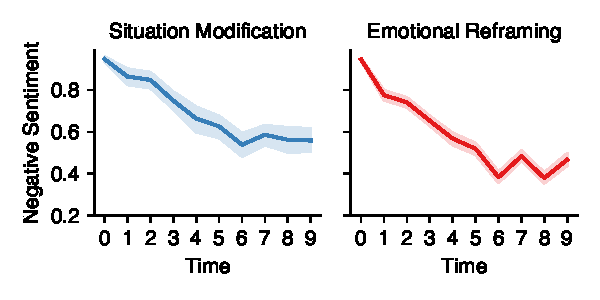
\includegraphics[width=\linewidth]{figure/sentiment.pdf}
    \caption{Negative sentiment decreased over the span of the conversation. Shaded area represents bootstrapped 95\% confidence intervals. Ns = 405 and 2052 conversations for situation modification and emotional reframing. The correlations between turn number and time bins is -.33 and .39 for Situation Modification and Emotional reframing. If we do this within person (as I think we should), the correlations are weaker: -.07 and -.36, respectively.}
    \label{fig:sentiment}
\end{figure}

\begin{figure}
    \centering
    \includegraphics[width=\linewidth]{figure/wordclouds.pdf}
    \caption{Word clouds from TF-IDF vectorization of user and bot text from situation modification and emotional reframing interventions.}
    \label{fig:wordclouds}
\end{figure}



\section*{Discussion} 

In this investigation, we deployed two motivational support chatbots---based on situation modification and emotional reframing---for a year on Khan Academy. 
To measure their impact, we compared user behavior before and after exposure to the chatbot intervention.
Because users chose when to use the chatbots, we used Bayesian IRT to account for potential time-varying confounds.
After these adjustments, we found that studnets who engaged with either prompt worked for longer after having used the chatbots, attempted more items, and attempted more difficult items.
However, these immediate behavioral changes did not translate into performance changes immediately.
Students did not perform significantly better after engaging with the chatbots.

Why did these AI-mediated interventions improve persistence?
Prior research suggests that these process model based strategies help.
In one experiment, students asked to study with their phones further away from them received higher grades in subsequent tests (CHECK).
In another, providing students with the reframe that mistakes are a part of learning and not indicative of their worth also increased persistence. 
While expected for emotional reframing, our results suggest that situation modification might also be effective because of reductions in negative affect.
Future research should confirm the relative increases in persistence of situation modification stratetegies due to reductions in negative affect.

If these results hold, they offer important implications for the deployment of positive online behaviors.
First, is the idea that AI-chatbots, when adequately prompted can work like motivational coaches.
Just like tutors and mentors help people with the challenges that occurr when things are difficult, complicated, or frustrating, AI-chatbots can help users deal with these difficulties.
This can result in increased persistence in positive behaviors that would otherwise be ended.

Lower-skill learners may require more than motivational support alone.
Exploratory analyses indicated that students with lower baseline skill did not benefit from chatbot exposure [CITE].
This pattern suggests that for these learners, motivational prompts should be paired with content-focused scaffolds (e.g., targeted hints, worked examples, or prerequisite review): increased effort is unlikely to yield gains when essential knowledge is missing.

\subsection*{Future Directions}

There are several limitations of this study that are worth highlighting. 
First and foremost, the highly naturalistic setting in which we collected the data meant that we were unable to randomly assign users to condition, weakening the causal interpretation of these findings.
That said, the pattern of behavior prior to exposure to the chatbots does not suggest that regression to the mean is a viable explanation for these findings.
And we capitalized on the temporal resolution of the data to control for two crucial time-varying confounds: user motivation/skill and item difficulty.
If these findings replicate in controlled experiments, we can have more faith that AI-based motivational coaches can increase persistence in difficult tasks.

A second limitation is generalizability.
We tested these motivational coaches in the context of online learning in the Khan Academy platform.
For the most part, this means school aged children working on math.
It is unclear how well these kinds of AI motivational coaches would translate to other kinds of important but tedious tasks, and other kinds of users.
For instance, could these kinds of motivational AI agents help users navigate adult tasks like filing taxes, or investing for retirement?
Future studies could address these possibilities.

Finally, measuring changes in skill is difficult.
Better measures and a more intentional design might have allowed us to better understand how AI motivational coaches could improve performance.
With the crude measurement of percent correct, we were unable to find robust effects on performance.

Future work can capitalize on these opportunities. 
First, testing motivational AI coaches with randomized experiments is crucial to establish causality, and better test the mechanism of the reduction of negative emotion.
Second, our setup allowed us only to make one intervention available, and then the other. 
Future research could address the possibility of personalization and targeted deployment.
For instance, user behavior and contents of the conversation with the AI tutor (i.e., Khanmigo) could be mined to proactively detect when students might benefit from receiving this intervention.
Likewise, the content of the intervention itself could be tailored, such that students who need a situation modification intervention get that, and students who at some other point need some other thing (e.g., a growth mindset intervention), get that.
Finally, the longer term effects of using AI motivational coaches shoudl be studied.


\subsection*{Conclusion}
Taken together, this study offers large-scale evidence from a high-stakes, ecologically valid setting that AI-delivered, theory-based motivational prompts can meaningfully boost persistence and encourage learners to attempt more challenging material—without external prodding. 
Because participation was entirely self-initiated, the findings speak to the potential of interventions that learners actively choose rather than ones imposed on them. At the same time, the skill-contingent nature of performance gains underscores a key design principle: pair motivational coaching with targeted instructional scaffolding. 
As digital learning and professional training increasingly integrate AI, embedding emotion-regulation supports represents a practical, scalable, and learner-driven approach to fostering sustained engagement in contexts where it matters most.


\section*{Methods}

\subsection*{Setting and data}
We analyzed de-identified platform logs from Khan Academy over a one-year period (January–December 2024).
Two motivational support chatbots grounded in the process model of emotion regulation were available within the product: \emph{Situation Modification} (SM) and \emph{Emotional Reframing} (ER).
Each exposure was user-initiated via an on-screen prompt (Figure~\ref{fig:interface}); no pop-up or forced assignment was used.
Logs include time-stamped item attempts (start/end times, correctness) and chatbot conversation text for users who chose to interact.

\subsection*{Participants}
The analytic sample comprised approximately 4{,}000 unique learners who engaged with at least one of the two chatbots during the study window and who had activity in both the pre- and post-exposure windows defined below.
We included the first qualifying exposure per user per condition (SM and ER analyzed separately).
Users without activity in either the pre- or post-window were excluded from the corresponding analysis.
All data were de-identified prior to analysis.

\subsection*{Interventions}
The SM chatbot encouraged users to structure their environment or routines to reduce reliance on willpower (e.g., minimizing distractions, planning short focused sessions).
The ER chatbot helped users reinterpret frustration and mistakes as expected, informative signals of learning progress.
Both prompts were delivered via a short, text-based exchange that adapted to user inputs; no content tutoring was provided.

\subsection*{Design and exposure definition}
Because use of the chatbots was self-initiated, we adopted a within-learner pre/post design with fixed effects and calendar-time controls.
For each user’s first exposure in a condition, we defined a pre-exposure window as the 7 days preceding the exposure (days \([-7,-1]\)) and a post-exposure window as the 7 days following the exposure (days \([+1,+7]\)).
To avoid contaminating post measures with the triggering session, we excluded activity from the exposure session itself (day 0) in primary analyses.
We computed outcomes within each window and compared post versus pre, controlling as described below.

\subsection*{Measures}
\textbf{Engagement (primary).} Total time on task during the window, log-transformed for analysis. Time on task was computed from item start/end timestamps after trimming extreme durations at conventional percentiles.

\textbf{Challenge-seeking (secondary).} Average difficulty of items attempted during the window. Difficulty parameters were obtained from an item-response model described below and scaled so that higher values indicate more difficult items.

\textbf{Performance (primary).} Percentage of correct responses during the window. As a complementary specification, we also analyzed time-varying IRT ability (``skill'') estimates.

\subsection*{Item and learner latent traits}
We estimated time-varying learner skill and motivation and item difficulty using a Bayesian model at the attempt level (equations in the main text).
Let \(s\) index learners, \(i\) items, and \(t\) ordered attempts. We modeled log-duration and correctness jointly:
\begin{align*}
    \text{Log-durations}_{s,i,t} &\sim \mathcal{N}(\mu_{\text{duration}}, \, \sigma_{\text{duration}}),\\
    \mu_{\text{duration}} &= \text{difficulty}_i + \text{motivation}_{s,t} - \text{skill}_{s,t},\\
    p(\text{Correct}_{s,i,t}=1) &= \sigma(\text{skill}_{s,t} - \text{difficulty}_i + \text{motivation}_{s,t}).
\end{align*}
Latent skill and motivation followed separate Gaussian random walks with exponential priors on their step sizes; item difficulties had hierarchical Gaussian priors. Posterior summaries (posterior means) for skill, motivation, and item difficulty were carried forward into the outcome models.

\subsection*{Statistical analysis}
Primary analyses were estimated separately for SM and ER.
We fit linear models at the user\,\(\times\,\)window level with user fixed effects and calendar-week fixed effects. For engagement we modeled log time on task; for challenge-seeking, average item difficulty; and for performance, percent correct. All models included time-varying skill and (when relevant) the average item difficulty in the window as covariates. Standard errors were clustered at the user level.

As robustness checks, we (i) excluded the 24 hours before and/or after exposure; (ii) varied the window length (3, 7, 14 days); (iii) re-estimated effects at the attempt level with user fixed effects; (iv) examined the second exposure to assess attenuation; and (v) repeated the performance analysis using IRT skill as the outcome.
Heterogeneity analyses tested moderation by baseline skill (pre-exposure skill) and gender when available.

\subsection*{Ethical considerations}
Analyses were conducted on de-identified data provided under a data-use agreement with Khan Academy.
This research protocol was reviewed and determined \emph{[exempt/approved—fill in]} by the \emph{[IRB name—fill in]} (Protocol \emph{[ID—fill in]}).
No interventions were randomized by the researchers; chatbot use was voluntary and user-initiated within the platform.

\subsection*{Pre-registration}
Analyses, primary/secondary outcomes, and exclusion rules were preregistered prior to data analysis at \url{[link-to-preregistration]}.
Any deviations from the preregistered plan are noted in the Appendix.


\chapter{Using Artificial Intelligence to Assess Personal Qualities in College Admissions}

Personal qualities like prosocial purpose and leadership predict important life outcomes, including college success. Unfortunately, the holistic assessment of personal qualities in college admissions is opaque and resource-intensive. Can artificial intelligence (AI) advance the goals of holistic admissions? While cost-effective, AI has been criticized as a “black box” that may inadvertently penalize already disadvantaged subgroups when used in high-stakes settings. Here we consider an AI approach to assessing personal qualities that aims to overcome these limitations. Research assistants and admissions officers first identified the presence/absence of seven personal qualities in \textit{n} = 3,131 applicant essays describing extracurricular and work experiences. Next, we fine-tuned pretrained language models with these ratings, which successfully reproduced human codes across demographic subgroups. Finally, in a national sample (\textit{N} = 309,594), computer-generated scores collectively demonstrated incremental validity for predicting six-year college graduation. We discuss challenges and opportunities of AI for assessing personal qualities.


\section*{Introduction}

Many colleges embrace the ideals of holistic review. In a recent survey by the National Association for College Admissions Counseling, 70\% of admissions officers said they consider personal qualities to be an important factor when selecting applicants \cite{national_research_council_assessing_2011}. This aim is justified by longitudinal research affirming that personal qualities—whether referred to as “non-cognitive skills,” “social-emotional competencies,” “personality,” or “character”—predict positive life outcomes in general and success in college in particular 
 \cite{moffitt_gradient_2011, almlund_personality_2011, robbins_psychosocial_2004, kyllonen_personality_2014}. Moreover, a holistic admissions process can advance equity, some argue, as applicants are able to demonstrate qualifications not reflected in their standardized test scores, which tend to be highly correlated with socioeconomic advantage \cite{coleman_understanding_2018}.

However, history shows that equity is certainly not guaranteed by holistic review. A century ago, Columbia University first began requiring applicants to write a personal essay, which admissions officers evaluated for evidence of “good character” 
 \cite{karabel_chosen_2005}. Previously, the university’s admissions decisions had been based primarily on standardized test scores. The result was a growing proportion of Jewish students in each entering class, which in turn led to concerns that, as Columbia’s dean at the time put it, the campus was no longer welcoming to “students who come from homes of refinement” (p. 87). It has been argued that for Columbia and other Ivy League colleges in that era, not requiring the justification, explanation, or even disclosure of these summary character judgments enabled the unfair exclusion of qualified Jewish applicants.
 
 %anti-Semitic admissions were able to unfairly penalize Jewish applicants because the process by which admissions officers arrived at summary judgments of character was not disclosed. 

Although its aims may be nobler today, the holistic review process itself remains much the same. Admissions officers still rely heavily on the personal essay to evaluate an applicant’s personal qualities \cite{national_research_council_assessing_2011}. The particulars of how, or even which, personal qualities are assessed, remain undisclosed to either applicants or the public, and even the “admissions officers themselves simply do not have a common definition of holistic review beyond 'reading the entire file'” \cite{bastedo_what_2018}. As one admissions officer put it, the status quo of holistic review is both ``opaque and secretive \cite{starkman_confessions_2013}.''

Recently, a more transparent and systematic process has been recommended for the holistic review of personal qualities in college admissions. Specifically, admissions officers have been urged to assess individual personal qualities separately (as opposed to making a summary judgment of “good character”), to use structured rubrics (as opposed to intuition), and to carry out multiple, independent evaluations (as opposed to relying on a single officer’s judgment) \cite{coleman_understanding_2018,anderson_character_2020}. Such recommendations represent the application of basic psychometric principles and, in research contexts, have long been used to increase the reliability, validity, and interpretability of human ratings \cite{kahneman_noise_2021,rushton_behavioral_1983}. Moreover, the transparency of this systematic approach should limit bias—whether accidental or intentional. 

In college admissions, however, this ideal is hardly ever achieved. The soaring number of applications that admissions officers must review—which for the majority of colleges has more than doubled in the last two decades—affords extraordinarily limited time to review each one \cite{hoover_working_2017,korn_elite_2018}. These logistical and budgetary constraints are likely to continue to prohibit the implementation of best practices that, were resources unlimited, could optimize reliability, validity, interpretability—and in turn, equity.

Can artificial intelligence (AI) advance the aims of holistic review? With stunning efficiency, AI systems identify patterns in data and, with stunning fidelity, apply learned models to new cases. For example, a computer algorithm could be trained to generate personal quality scores from student writing instantaneously, reliably, and at near-zero marginal cost. However, there are concerns that the “black box” of an AI algorithm may inadvertently perpetuate, or even exacerbate, bias against disadvantaged subgroups \cite{tay_conceptual_2022,hickman_automated_2022}. Such bias has been shown in the domains of hiring, criminal justice, and medical diagnosis \cite{manyika_what_2019, obermeyer_dissecting_2019, ensign_runaway_2018}. In college admissions, AI-quantified essay content and style have been shown to correlate more strongly with household income than do SAT scores \cite{alvero_essay_2021}. Opaque AI algorithms that provide fertile ground for bias recall the anti-Semitic holistic review practices of a century ago. %Arguably, by allowing bias to remain hidden, any “black box” process can undermine, rather than advance, equitable decision making.

Efforts within the AI community to address these issues have given rise to concepts such as Human-Centered AI \cite{riedl_humancentered_2019, shneiderman_human-centered_2020} and Explainable AI \cite{gunning_xaiexplainable_2019}. 
These frameworks emphasize alignment with stakeholder objectives, interpretability, and equity---while promoting the idea of automation as a complement rather than a substitute for human control \cite{shneiderman_human-centered_2020}. 
    Rather than simply maximizing predictive accuracy, these approaches prioritize alignment with stakeholder goals (e.g., admitting students who demonstrate prosocial purpose, \cite{noauthor_our_2021}), interpretability (e.g., providing separate, face-valid scores for separate personal qualities rather than a single summary score of character with no evidence of face validity), and rigorously auditing model outputs for unintended bias. By prioritizing these aspects, digital technology can facilitate the identification of discrimination and contribute to rectifying historical exclusion \cite{lobel_equality_2022}.

In this investigation, we developed an artificial intelligence (AI) approach to assessing personal qualities with these priorities in mind. 
We began with a de-identified sample of 309,594 college applications (see \textbf{Figure 1}). Each included a 150-word essay describing an extracurricular or work activity of the applicant’s choice. Next, in a \textit{Development Sample} of 3,131 essays, research assistants (RA) and admissions officers (AO) identified the presence or absence of seven different personal qualities commonly valued by universities and shown in prior research to predict college success \cite{almlund_personality_2011}. See \textbf{Table 1}. Research assistant and admissions officer ratings were used to fine-tune separate RoBERTa language models \cite{liu_roberta_2019} for each personal quality. We then confirmed each model’s interpretability as well as evidence of convergent, discriminant, and predictive validity by demographic subgroup. Finally, we applied these fine-tuned models to the \textit{Holdout Sample} of 306,463 essays, examining associations between computer-generated personal quality scores, demographic characteristics, and six-year college graduation.

\begin{table*}
\small
\caption{Personal qualities and example essay excerpts}
\def\arraystretch{1}%  1 is the default, change whatever you need
\begin{tabular}{  p{.275\linewidth}  p{.675\linewidth}}
\hline
% Personal quality: Criteria for coding by human raters & Fictionalized example essay with relevant phrases in italics\\                                                                      
\multicolumn{1}{c}{\textbf{Personal quality}} & \multicolumn{1}{c}{\textbf{Fictionalized excerpts}}\\                                                                      \hline
\textbf{Prosocial purpose}

Helping others, wanting to help others, considering the benefits to others, mentioning reasons for helping others, or reflecting on how enjoyable or rewarding it is to help others. & Every summer for the last three years, I worked as camp counselor at a camp for young children from underprivileged families. Helping children realize their hidden talents is one of the most rewarding experiences I have ever had. I’ve been so fulfilled by watching these children develop confidence in their abilities. This experience has been so important to me, and it showed me that a career in education is where I belong.                                         \\ \\
\textbf{Leadership}

Serving in a leadership role, commenting on what he or she did in his or her capacity as a leader, or discussing the value, meaning, or importance of leadership.                            & I was chosen to be cheerleading captain during my senior year. My freshman year captain had a huge impact on my life, and I felt like it was my time to pay it forward. I am so proud of everything I did for the girls: creating a mentorship system, organizing events and fundraisers, and encouraging everyone to work as hard as they could. At the end of the year, a few girls thanked me. I was completely overcome with emotion. I’ve never felt so gratified in my life. \\ \\
\textbf{Learning}

Improving, learning, or developing knowledge, skills, or abilities.                                                                                                                       & I played softball in high school. When I started, I was not a very strong player. When I finally made the varsity team my senior year, I was determined to have a better season. I worked constantly to improve my game – during practice and on my own time. My skills grew so much. Because of my hard work, I finished the year with the best record on my team!                                                                                                                \\ \\
\textbf{Goal pursuit}

Having a goal and/or a plan.                                                                                                                                                              & I have been playing soccer since I was six years old. Unfortunately, last year I injured my knee, and it has been a struggle to get back to the level I was playing at before my injury. It has been really challenging, but I’ve been doing physical therapy and practicing everyday so that I can be a varsity starter this year.                                                                                                                                                \\ \\
\textbf{Intrinsic motivation}

Describing the activity as enjoyable or interesting. Liking the activity or identifying with it.                                                                                         & Running track is so much more than a sport to me. It’s a challenge and an adventure, and I put everything I have into it. I love every aspect of it, even the afternoons I spend drenched in sweat in the scorching heat.                                                                                                                                                                                                                 \\ \\
\textbf{Teamwork}

Working with or learning from others. Valuing what fellow participants bring to the activity.                                                                                            & I’ve been on my school’s debate team since my freshman year, and was elected co-captain because of my commitment to the team’s success. My fellow co-captains and I worked together to get our team ready for competitions. We knew that a strong team performance was more important than the successes of a few individuals. We stressed teamwork and cooperation between our teammates. Because we focused on team effort, we earned first place at the state meet.             \\ \\
\textbf{Perseverance}

Persisting in the face of challenge.                                                                                                                                                      & I’ve learned to become a gracious victor and to grow from defeat. Track has helped me overcome my fear of losing, and even helped me put my life in perspective. I’ve learned to keep working and fighting even when the odds seem impossible to beat. There were many times that I found myself lagging, but I pulled ahead at the end because I never gave up. The most important thing I’ve learned is to never let anything stand in my way.     \\                         \hline    
\multicolumn{2}{l}{\textit{Note.} Our data use agreement with Common App does not allow us to publish real excerpts to protect student identity.}
\end{tabular}
\end{table*}

\begin{figure*}
    \centering
    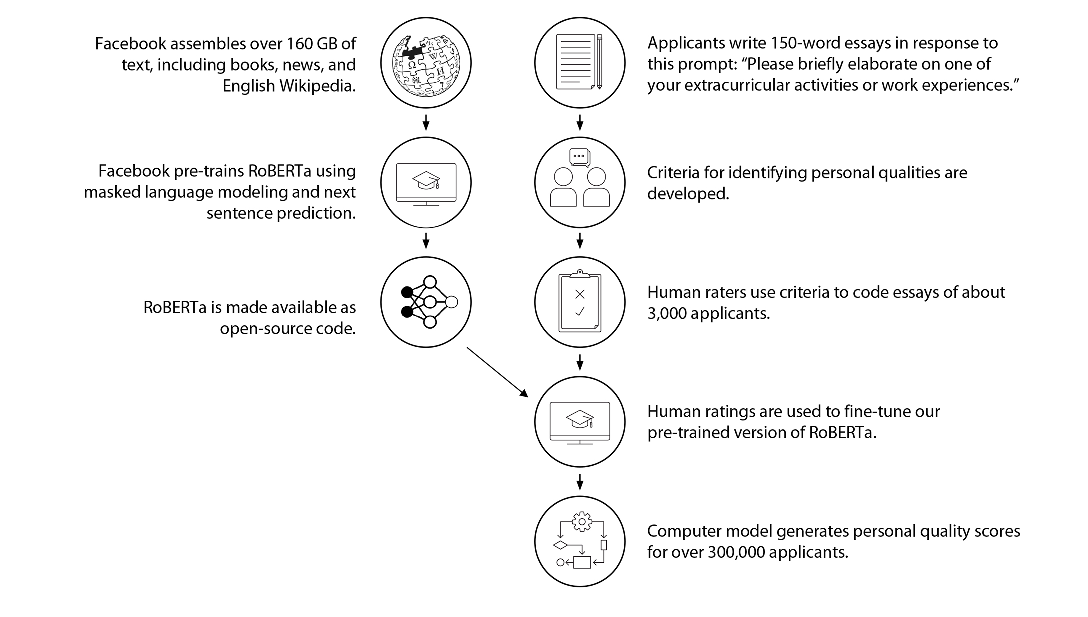
\includegraphics[width= \textwidth]{fig1_new2_scale.pdf}
    \caption{An artificial intelligence approach to assessing personal qualities in college admissions.}
    \label{fig:f1}
\end{figure*}

\begin{landscape}
\begin{table*}
\centering
\caption{Descriptive statistics and correlations between human ratings and computer-generated likelihoods of personal qualities in the Development Sample}
\begin{tabular}{@{\extracolsep{3pt}}lD{.}{.}{1.2}D{.}{.}{1.2}D{.}{.}{1.2}D{.}{.}{1.2}D{.}{.}{1.2}D{.}{.}{1.2}D{.}{.}{1.2}D{.}{.}{1.2}D{.}{.}{1.2}D{.}{.}{1.2}D{.}{.}{1.2}D{.}{.}{1.2}D{.}{.}{1.2}D{.}{.}{1.2}}
\hline
& \multicolumn{7}{c}{Research Assistant Ratings}& \multicolumn{7}{c}{Admissions Officer Ratings}\\
\cmidrule{2-8}\cmidrule{9-15}
Personal Quality & \multicolumn{1}{c}{PP} & \multicolumn{1}{c}{LD} & \multicolumn{1}{c}{TW} & \multicolumn{1}{c}{LR} & \multicolumn{1}{c}{PS} & \multicolumn{1}{c}{IM} & \multicolumn{1}{c}{GP}& \multicolumn{1}{c}{PP} & \multicolumn{1}{c}{LD} & \multicolumn{1}{c}{TW} & \multicolumn{1}{c}{LR} & \multicolumn{1}{c}{PS} & \multicolumn{1}{c}{IM} & \multicolumn{1}{c}{GP}\\\hline
Computer-Generated Likelihoods        & \multicolumn{1}{l}{} & \multicolumn{1}{l}{} & \multicolumn{1}{l}{} & \multicolumn{1}{l}{} & \multicolumn{1}{l}{} & \multicolumn{1}{l}{} & \multicolumn{1}{l}{}& \multicolumn{1}{l}{} & \multicolumn{1}{l}{} & \multicolumn{1}{l}{} & \multicolumn{1}{l}{} & \multicolumn{1}{l}{} & \multicolumn{1}{l}{} & \multicolumn{1}{l}{} \\
\hspace{1em}1. Prosocial purpose (PP) &  .86\text{***} & -.01  & -.04\text{*} & -.09\text{***} & -.12\text{***} & -.05\text{**} &  .04\text{*}  &  .80\text{***} & -.13\text{***}  & .13\text{***} & -.22\text{***} & -.24\text{***} & -.09\text{**} &  -.19\text{***}  \\ 
\hspace{1em}2. Leadership (LD) & -.01  &  .81\text{***} &  .15\text{***} & -.01  &  .00  & -.09\text{***} &  .05\text{**}& .13\text{***}  &  .73\text{***} &  .16\text{***} & -.15\text{***}  &  -.06\text{***}  & -.16\text{***} &  .01\\ 
\hspace{1em}3. Teamwork (TW) & -.07\text{***} &  .18\text{***} &  .62\text{***} &  .06\text{**} &  .07\text{***} & -.02  &  .06\text{**}& -.18\text{***} &  .16\text{***} &  .62\text{***} &  .07\text{***} &  .10\text{***} & -.03  &  .10\text{***} \\ 
\hspace{1em}4. Learning (LR) & -.10\text{***} & -.05\text{**} &  .04\text{*} &  .77\text{***}&  .11\text{***} & -.01  & -.03& -.28\text{***} & -.15\text{***} &  -.07\text{***} &  .65\text{***}&  .07\text{***} & .01  & .09\text{***}  \\ 
\hspace{1em}5. Perseverance (PS) & -.16\text{***} & -.01  &  .06\text{**} &  .10\text{***} &  .67\text{***}&  .03 &  .05\text{**}& -.35\text{***} & -.10\text{***}  &  .11\text{***} &  .08\text{***} &  .48\text{***}&  .09\text{***} &  .26\text{***} \\ 
\hspace{1em}6. Intrinsic motivation (IM) & -.05\text{**} & -.09\text{***} &  .00  & -.03 &  .04\text{*} &  .73\text{***} &  .03 & .08***\text{**} & -.24\text{***} &  -.08\text{***}  & -.01 &  .08\text{***} &  .45\text{***} &  -.05\text{***} \\ 
\hspace{1em}7. Goal pursuit (GP) &  .06\text{***} &  .06\text{**} &  .06\text{***} & -.01  &  .02  &  .02  &  .59\text{***}&  -.31\text{***} &  -.05\text{**} &  .12\text{***} & .15\text{***}  &  .27\text{***}  &  .06\text{***}  &  .45\text{***}\\ \hline
Descriptive Statistics                & \multicolumn{1}{l}{} & \multicolumn{1}{l}{} & \multicolumn{1}{l}{} & \multicolumn{1}{l}{} & \multicolumn{1}{l}{} & \multicolumn{1}{l}{} & \multicolumn{1}{l}{}& \multicolumn{1}{l}{} & \multicolumn{1}{l}{} & \multicolumn{1}{l}{} & \multicolumn{1}{l}{} & \multicolumn{1}{l}{} & \multicolumn{1}{l}{} & \multicolumn{1}{l}{} \\
\hspace{1em}Human Inter-Rater Reliability & .83 & .78 & .61 & .73 & .66 & .63 & .57& .60 & .49 & .30 & .31 & .24 & .23 & .15 \\ 
\hspace{1em}Frequency of Human Rating & .34 & .18 & .26 & .42 & .19 & .42 & .31& .28 & .25 & .22 & .44 & .21 & .41 & .25\\ 
\hspace{1em}Mean of Computer-Generated Likelihood & .36 & .19 & .26 & .45 & .19 & .45 & .32& .30 & .25 & .22 & .46 & .24 & .42 & .25 \\ 
\hline
\multicolumn{15}{p{17.25cm}}{\textit{Note.} Inter-rater reliability for human raters was measured with Krippendorf’s alpha. Correlations between human ratings and computer-generated likelihoods for the same personal qualities are shown along the diagonals. All correlations are point-biserial correlation coefficients between binary human ratings and continuous computer-generated likelihoods. \text{*} \textit{p} < .05. \text{**} \textit{p} < .01. \text{***} \textit{p} < .001. \textit{n} = 3,131. \textit{n} for inter-rater reliability = 206 essays coded by multiple research assistants, n = 3131 essays coded by two admission officers.}
\end{tabular}
\end{table*}
\end{landscape}
\section*{Results}

On average, research assistants and admissions officers found evidence for two out of seven personal qualities in each essay. As shown in \textbf{Table 2}, some personal qualities were more commonly observed than others. For instance, research assistants and admissions officers identified leadership in 42\% and 44\% of essays, respectively; in contrast, they identified perseverance in only 19\% and 21\% of essays, respectively. Correlations between research assistant and admission officer ratings ranged between $\phi$ = .193 and .703, \textit{p}s < .001.

Using these binary human ratings, we fine-tuned separate RoBERTa models to produce continuous likelihood scores for each personal quality, and each kind of rater. See \textbf{Section 2} in \textbf{Supplementary Materials} for details on model pretraining and fine-tuning.

\subsection*{Model interpretability}
We used the \textit{transformers-interpret} package \cite{pierse_transformers_2021,janizek_explaining_2020} to identify the words (or fractions of words) that these fine-tuned RoBERTa models relied on most to generate personal quality scores. 
%generate attribution scores for each essay. Each token (i.e., word or fraction of word) receives a score indicating how relevant this feature is for generating likelihoods for each personal quality. For each personal quality, we averaged the scores for each word across essays and found the words the model relied on for generating the corresponding likelihoods. 
As shown in \textbf{Figure \ref{fig:interpret},} there was reasonable evidence of face validity. For instance, RoBERTa assigned higher scores for leadership when essays mentioned ``president,'' ``leader,'' and ``captain.'' Models trained on admission officer ratings produced similar attribution scores: average word-level attribution scores correlated between .392 and .983, \textit{p}s < .001.
See \textbf{Section 7} in \textbf{Supplementary Materials} for details.

\begin{figure*}
    \centering
    \includegraphics[width = \textwidth]{fig2.jpg}
    \caption{Complete or partial words on which RoBERTa models finetuned on research assistants relied most for generating personal quality scores. Font size is proportional to word importance.  Darker words are more common. Token ``gru'' is a fraction of the word ``grueling'', Token ``unte'' is a fraction of the word ``volunteer''. 
    Words importance is not invariant across essays, it depends on word context.
    Word importance and frequency were largely independent (\textit{r} = -.03, p < .001). For instance, for intrinsic motivation, the model relied more on the word ``pleasure'' then the word ``fun,'' but essays were more likely to contain the word ``fun'' then the word ``pleasure.''}
    \label{fig:interpret}
\end{figure*}


\subsection*{Convergent and discriminant validity of computer-generated likelihoods in the Development Sample}
Computer-generated likelihoods for each personal quality converged with human ratings of the same personal quality (\textit{r}s ranged from .59 to .86, average \textit{r} = .74, for research assistants; \textit{r}s ranged from .45 to .80, average \textit{r} = .62, for admission officers). In contrast, computer-generated likelihoods for a particular personal quality did not correlate with human ratings of other personal qualities (\textit{r}s from -.16 to .18, average \textit{r} = .01, for research assistants; \textit{r}s from -.35 to .27, average \textit{r} = -.03, for admission officers). See \textbf{Table 2}. Unsurprisingly, the more reliably human raters were able to code each personal quality, the better the computer-generated likelihoods of personal qualities matched these ratings (\textit{r} = .95, \textit{p} = .001, for research assistants; \textit{r} = .94, \textit{p} = .001, for admission officers). In the sub-sample of essays that were coded by multiple raters, model scores correlated more strongly with human ratings than human ratings correlated with each other (\textit{M}$_{human-computer}$ = .74, \textit{M}$_{human-human}$ = .69, \textit{t} = 4.16, \textit{p} = .006, for research assistants; \textit{M}$_{human-computer}$ = .60, \textit{M}$_{human-human}$ = 0.28, \textit{t} = 19.40, \textit{p} < .001, for admissions officers). There were positive correlations between computer-generated likelihoods for personal qualities from models trained on research assistants and admissions officers (\textit{r}s ranged from .394 to .869, \textit{p}s < .001).

\subsection*{Convergent validity does not vary by demographic subgroup in the Development Sample}

Correlations between human ratings and computer-generated likelihoods of personal qualities were similar across subgroups. For example, the average correlation between human-rated and computer-generated personal quality scores was .74 for female applicants and .73 for male applicants, for research assistants. The pattern of results was equivalent for admission officers. As shown in \textbf{Tables S11 and S12}, \added{after correcting for multiple comparisons \cite{benjamini_control_2001},} 13\% and 9\% of the correlations differed by subgroup for research assistants and admissions officers, respectively. In about half of these comparisons, the models were more accurate for the marginalized group, while in the other half, the majority subgroup was favored. \added{In most of these cases the difference between the correlations was not very large (mean $|\Delta r_{RA}|$ = .054, range of $\Delta r_{RA}$ = -.121 -- .056), mean $|\Delta r_{AO}|$ = .10, range of $\Delta r_{AO}$ = -.206 -- .123).}

% \begin{table}
% \centering
% \caption{Odds ratios from binary logistic regression models predicting six-year college graduation in the \textit{N} = 306,463 Holdout Sample}
% % \begin{tabular}{@{\extracolsep{3pt}}lD{.}{.}{2.3}D{.}{.}{2.3}D{.}{.}{2.3}D{.}{.}{2.3}}
% \begin{tabular}{@{\extracolsep{3pt}}lcccc}
% \hline
% & \multicolumn{2}{c}{Research Assistant}          & \multicolumn{2}{c}{Admission Officer}\\
% \cmidrule{2-3}\cmidrule{4-5}
% \multicolumn{1}{c}{}          & \multicolumn{1}{c}{(1)} & \multicolumn{1}{c}{(2)} & \multicolumn{1}{c}{(1)} & \multicolumn{1}{c}{(2)} \\\hline
% \multicolumn{5}{l}{Computer-generated likelihoods of personal qualities}\\
% \hspace{1em}Prosocial purpose& 1.132^{***} & 1.075^{***}& 1.252^{***} & 1.116^{***} \\ 
%   & (0.005) & (0.005)& (0.006) & (0.006) \\ 
% \hspace{1em}Leadership & 1.133^{***} & 1.065^{***}& 1.214^{***} & 1.084^{***} \\ 
%   & (0.005) & (0.005)& (0.005) & (0.005) \\ 
% \hspace{1em}Teamwork & 1.080^{***} & 1.031^{***} & 1.135^{***} & 1.062^{***} \\ 
%   & (0.005) & (0.005)  & (0.005) & (0.005) \\ 
% \hspace{1em}Learning & 1.065^{***} & 1.045^{***}& 1.146^{***} & 1.034^{***} \\ 
%   & (0.004) & (0.005)& (0.005) & (0.005) \\ 
% \hspace{1em}Perseverance & 1.071^{***} & 1.012^{**}& 1.089^{***} & 1.047^{***} \\ 
%   & (0.005) & (0.005)& (0.005) & (0.006) \\ 
% \hspace{1em}Intrinsic motivation  & 1.068^{***} & 1.007& 1.142^{***} & 1.009 \\ 
%   & (0.004) & (0.005)& (0.005) & (0.005) \\ 
% \hspace{1em}Goal pursuit & 1.041^{***} & 1.005 & 1.048^{***} & 1.030^{***} \\ 
%   & (0.004) & (0.005) & (0.005) & (0.005) \\ 
% Race/ethnicity (vs. white) & & & \\
% \hspace{1em}Black  & & 0.774^{***}& & 0.775^{***} \\
%   & & (0.019)& &(0.019) \\
% \hspace{1em}Latino& & 0.871^{***}& & 0.868^{***} \\
%   & & (0.019)&  & (0.019) \\
% \hspace{1em}Asian & & 0.735^{***}& & 0.739^{***} \\
%   & & (0.017)  &  & (0.017) \\
% \hspace{1em}Other & & 0.749^{***}& & 0.750^{***} \\
%   & & (0.017)&  & (0.017) \\
% \hspace{1em}No race reported  & & 0.849^{***}& & 0.853^{***} \\
%   & & (0.013)&  & (0.013) \\
% \multicolumn{5}{l}{Parental education (vs. No parent w/ college degree)} \\
% \multicolumn{2}{l}{\hspace{1em}One parent w/ college degree}  & 1.199^{***}& & 1.198^{***} \\
%   & & (0.012)&  & (0.012) \\
% \multicolumn{2}{l}{\hspace{1em}Two parents w/ college degree}  & 1.335^{***}& & 1.334^{***} \\
%   & & (0.012)&  & (0.012) \\
%   Female  &  & 1.435^{***}&  & 1.430^{***} \\ 
%   &  & (0.010)&  & (0.010) \\ 
% Married parents  &  & 1.311^{***}&  & 1.308^{***} \\ 
%   &  & (0.011)&  & (0.011) \\ 
% English language learner &  & 0.769^{***}&  & 0.774^{***} \\ 
%   &  & (0.015)&  & (0.016) \\ 
% Title 1 high school &  & 0.951^{***}&  & 0.947^{***} \\ 
%   &  & (0.013)&  & (0.013) \\ 
% Out-of-school activities (OSA) &  &  & & \\
% \hspace{1em}Number of OSA &  & 1.250^{***}&  & 1.241^{***} \\ 
%   &  & (0.005)&  & (0.005) \\
% \hspace{1em}Time per OSA&  & 1.088^{***}&  & 1.083^{***} \\ 
%   &  & (0.004)&  & (0.004) \\
% \hspace{1em}Proportion sports  &  & 1.042^{***}  &  & 1.035^{***} \\ 
%   &  & (0.005)&  & (0.005) \\ 
% Standardized test scores &  & 1.489^{***} &  & 1.482^{***} \\ 
%   &  & (0.006)&  & (0.006) \\ 
% Constant & 3.555^{***} & 2.533^{***}& 3.585^{***} & 2.543^{***} \\ 
%   & (0.004) & (0.014)& (0.004) & (0.014) \\ \hline
% \textit{AUC} & .560 & .689& .576 & .690\\
% \hline
% \multicolumn{5}{l}{\textit{Note.} * \textit{p} < .05. ** \textit{p} < .01. *** \textit{p} < .001.}                                            
% \end{tabular}
% \end{table}

\begin{table}[!htbp]
\centering
\caption{Odds ratios from binary logistic regression models predicting six-year college graduation in the \textit{N} = 306,463 Holdout Sample}
\begin{tabular}{@{\extracolsep{3pt}}lcccc}
\hline
& \multicolumn{2}{c}{Research Assistant} & \multicolumn{2}{c}{Admission Officer} \\
\hline
& (1) & (2) & (1) & (2) \\
\hline
\multicolumn{5}{l}{Computer-generated likelihoods of personal qualities} \\
\hspace{1em}Prosocial purpose & 1.132\textsuperscript{***} & 1.075\textsuperscript{***} & 1.252\textsuperscript{***} & 1.116\textsuperscript{***} \\
& (0.005) & (0.005) & (0.006) & (0.006) \\
\hspace{1em}Leadership & 1.133\textsuperscript{***} & 1.065\textsuperscript{***} & 1.214\textsuperscript{***} & 1.084\textsuperscript{***} \\
& (0.005) & (0.005) & (0.005) & (0.005) \\
\hspace{1em}Teamwork & 1.080\textsuperscript{***} & 1.031\textsuperscript{***} & 1.135\textsuperscript{***} & 1.062\textsuperscript{***} \\
& (0.005) & (0.005) & (0.005) & (0.005) \\
\hspace{1em}Learning & 1.065\textsuperscript{***} & 1.045\textsuperscript{***} & 1.146\textsuperscript{***} & 1.034\textsuperscript{***} \\
& (0.004) & (0.005) & (0.005) & (0.005) \\
\hspace{1em}Perseverance & 1.071\textsuperscript{***} & 1.012\textsuperscript{**} & 1.089\textsuperscript{***} & 1.047\textsuperscript{***} \\
& (0.005) & (0.005) & (0.005) & (0.006) \\
\hspace{1em}Intrinsic motivation & 1.068\textsuperscript{***} & 1.007 & 1.142\textsuperscript{***} & 1.009 \\
& (0.004) & (0.005) & (0.005) & (0.005) \\
\hspace{1em}Goal pursuit & 1.041\textsuperscript{***} & 1.005 & 1.048\textsuperscript{***} & 1.030\textsuperscript{***} \\
& (0.004) & (0.005) & (0.005) & (0.005) \\
\multicolumn{5}{l}{Race/ethnicity (vs.\ white)} \\
\hspace{1em}Black &  & 0.774\textsuperscript{***} &  & 0.775\textsuperscript{***} \\
&  & (0.019) &  & (0.019) \\
\hspace{1em}Latino &  & 0.871\textsuperscript{***} &  & 0.868\textsuperscript{***} \\
&  & (0.019) &  & (0.019) \\
\hspace{1em}Asian &  & 0.735\textsuperscript{***} &  & 0.739\textsuperscript{***} \\
&  & (0.017) &  & (0.017) \\
\hspace{1em}Other &  & 0.749\textsuperscript{***} &  & 0.750\textsuperscript{***} \\
&  & (0.017) &  & (0.017) \\
\hspace{1em}No race reported &  & 0.849\textsuperscript{***} &  & 0.853\textsuperscript{***} \\
&  & (0.013) &  & (0.013) \\
\multicolumn{5}{l}{Parental education (vs.\ no parent w/ college degree)} \\
\multicolumn{2}{l}{\hspace{1em}One parent w/ college degree} & 1.199\textsuperscript{***} &  & 1.198\textsuperscript{***} \\
&  & (0.012) &  & (0.012) \\
\multicolumn{2}{l}{\hspace{1em}Two parents w/ college degree} & 1.335\textsuperscript{***} &  & 1.334\textsuperscript{***} \\
&  & (0.012) &  & (0.012) \\
Female &  & 1.435\textsuperscript{***} &  & 1.430\textsuperscript{***} \\
&  & (0.010) &  & (0.010) \\
Married parents &  & 1.311\textsuperscript{***} &  & 1.308\textsuperscript{***} \\
&  & (0.011) &  & (0.011) \\
English language learner &  & 0.769\textsuperscript{***} &  & 0.774\textsuperscript{***} \\
&  & (0.015) &  & (0.016) \\
Title 1 high school &  & 0.951\textsuperscript{***} &  & 0.947\textsuperscript{***} \\
&  & (0.013) &  & (0.013) \\
\multicolumn{5}{l}{Out-of-school activities (OSA)} \\
\hspace{1em}Number of OSA &  & 1.250\textsuperscript{***} &  & 1.241\textsuperscript{***} \\
&  & (0.005) &  & (0.005) \\
\hspace{1em}Time per OSA &  & 1.088\textsuperscript{***} &  & 1.083\textsuperscript{***} \\
&  & (0.004) &  & (0.004) \\
\hspace{1em}Proportion sports &  & 1.042\textsuperscript{***} &  & 1.035\textsuperscript{***} \\
&  & (0.005) &  & (0.005) \\
Standardized test scores &  & 1.489\textsuperscript{***} &  & 1.482\textsuperscript{***} \\
&  & (0.006) &  & (0.006) \\
Constant & 3.555\textsuperscript{***} & 2.533\textsuperscript{***} & 3.585\textsuperscript{***} & 2.543\textsuperscript{***} \\
& (0.004) & (0.014) & (0.004) & (0.014) \\
\hline
\textit{AUC} & .560 & .689 & .576 & .690 \\
\hline
\multicolumn{5}{l}{\textit{Note.}\enspace * \textit{p} < .05.\; ** \textit{p} < .01.\; *** \textit{p} < .001.} \\
\end{tabular}
\end{table}

\subsection*{Human ratings and computer-generated likelihoods were largely unrelated to demographics in the Development Sample}
Demographic characteristics were largely unrelated to personal qualities, whether assessed by human raters (mean |$\phi_{RA}$| = 0.02, mean |$\phi_{AO}$| = 0.03) or by computer algorithm (mean |$d_{RA}$| = 0.06, mean |$d_{AO}$| = 0.08). One exception is that female applicants were rated as more prosocial than male applicants ($\phi_{RA}$ = .13, $\phi_{AO}$ = .12 \textit{p} < .001 for human ratings, $d_{RA}$ = 0.26, $d_{AO}$ = .28, \textit{p} < .001 for computer-generated likelihoods, \textit{p}-values adjusted for multiple comparisons \cite{benjamini_control_2001})—in line with other research showing gender differences in prosocial motivation and behavior favoring women \cite{kamas_empathy_2021}. See \textbf{Table S5} in \textbf{Supplementary Materials} for details. 

\subsection*{Computer-generated likelihoods were as predictive of college graduation as human raters in the Development Sample}
To compare the predictive validity of the computer-generated likelihoods with human ratings, we ran two logistic regression models in which personal qualities predicted college graduation. The computer-generated likelihoods were slightly more predictive than the human ratings, but the difference in the AUCs was not significant ($AUC_{human}$ = .565, $AUC_{computer}$ = .574, $\Delta AUC$ = .009, \textit{p} = .274, for research assistants; $AUC_{human}$ = .587, $AUC_{computer}$ = .603, $\Delta AUC$ = .017, \textit{p} = .120, for admission officers). Coefficients were slightly larger for computer-generated likelihoods as compared to human ratings (\textit{t} = 2.33, \textit{d} = 0.882, \textit{p} = .059, for research assistants; \textit{t} = 3.89, \textit{d} = 1.469, \textit{p} = .008, for admissions officers).

\subsection*{Computer-generated likelihoods were largely independent of demographics but, in support of criterion validity, predicted graduation in the Holdout Sample}
Next, we applied the models fine-tuned on research assistants and admissions officers to the \textit{Holdout Sample} of 306,463 essays. \added{For both categories of models, reliability across models trained on different subsets of the data was high (range of Cronbach's $\alpha$ = .990 to .997, for research assistants; range of Cronbach's $\alpha$ = .988 to .998, for admission officers). Even when considering any two models, they were likely to produce similar results (average inter-model correlation ranged from .910 to .967 for research assistants, .896 to .978 for admission officers).} Correlations between computer-generated likelihoods for personal qualities from models trained on research assistants and admissions officers ranged from .418 to .896, \textit{p}s < .001.

As in the development sample, computer-generated likelihoods for personal qualities were similar across demographic subgroups (mean |$d_{RA}$| = 0.05, mean |$d_{AO}$| = 0.06). In contrast, and as expected, demographics were more strongly related to standardized test scores (mean |\textit{d}| = 0.38) and degree of participation in out-of-school activities (mean |\textit{d}| = 0.17). See \textbf{Tables S7} and \textbf{S10} in \textbf{Supplementary Materials} for details.

About 78\% of students in the \textit{Holdout Sample} graduated from college within 6 years. As shown in Model 1 in \textbf{Table 4}, computer-generated likelihoods for personal qualities were each modestly predictive of college graduation when controlling for each other (\textit{OR}s from 1.041 to 1.132, \textit{p}s < .001, \textit{AUC} = .560, for research assistants; \textit{OR}s from 1.048 to 1.252, \textit{p}s < .001, \textit{AUC} = .576, for admission officers). \added{To estimate a ceiling on how much the essays can predict subsequent college graduation, we trained a RoBERTa model to predict college graduation from students' responses. This model achieved an out-of-sample AUC of .626, suggesting that consistent with previous research \cite{alvero_essay_2021} essays do encode information predictive of graduation outside of personal qualities. The same procedure using personal qualities results in smaller out-of-sample AUCs ($AUC_{RA}$ = .557, $AUC_{AO}$ = .568). See \textbf{Section 8} in \textbf{Supplementary Materials} for details.}

As shown in Model 2 in \textbf{Table 4}, in the models trained on research assistants, five of seven personal qualities remained predictive of college graduation when controlling for each other, demographics, standardized test scores, and out-of-school activities (\textit{OR}s from 1.012 to 1.075, \textit{p}s < .01). In the models trained on admissions officers, six of seven personal qualities remained predictive (\textit{OR}s from 1.030 to 1.116, \textit{p}s < .01). See \textbf{Figure S2} in \textbf{Supplementary Materials} for details on imputation.

As a further test for fairness, we tested whether the predictive power of computer-generated likelihoods of personal qualities was equivalent across subgroups. We added interaction terms between each personal quality and standardized test scores and each demographic characteristic. After controlling for multiple comparisons \cite{benjamini_control_2001}, we confirmed that the predictive effect of personal qualities was equal across demographic subgroups. Comparatively, the predictive accuracy of standardized tests differed across subgroups (mean $|\beta|$ = -0.053). We also tested for differences in predictive validity in intersections of two demographic subgroups (e.g., Black English language learners, Women in title 1 high schools). There were no consistent or theoretically interpretable patterns in these intersectional analyses. See \textbf{Section 9} in \textbf{Supplementary Materials} for details.

\section*{Discussion}
In a national dataset of over 300,000 college applications, we evaluated an artificial intelligence approach to measuring personal qualities from student writing. Specifically, we fine-tuned RoBERTa language models using expert ratings of prosocial purpose, leadership, teamwork, learning, perseverance, intrinsic motivation, and goal pursuit, respectively, in applicants’ essays about their out-of-school activities. We found that these models demonstrated convergent, discriminant, and predictive validity---and this evidence was consistent across demographic subgroups. In addition, computer-generated scores were largely independent of demographics. 

In contrast, two prior studies found that AI-extracted admission essay content and style correlate with socioeconomic status. Alvero and colleagues \cite{alvero_essay_2021} found that students from wealthier families tend to write about certain essay topics (e.g., human nature), whereas disadvantaged students tend to write about others (e.g., tutoring groups).
Likewise, Pennebaker and colleagues \cite{pennebaker_when_2014} found that categorical words (e.g., articles, prepositions) versus dynamic words (e.g., pronouns, adverbs) in college essays correlate with parental education at \textit{r} = .22.
Why do our results differ? It seems likely that personal qualities are distributed more evenly across demographic subgroups than the topics students choose to write about or the words they use to do so. However, we cannot rule out methodological differences. Alvero et al. \cite{alvero_essay_2021} used essays from the University of California system, and Pennebaker et al. \cite{pennebaker_when_2014} used essays from a large state university. 
In contrast, our sample included a larger and more diverse set of public and private four-year colleges from across the United States. In addition, both of these prior studies used personal statements totaling several hundred words, whereas the essays to which we had access were a maximum of 150 words and focused specifically on extracurricular activities and work experiences. Finally, rather than using unsupervised topic modeling or dictionary approaches, we fine-tuned a language representation model using human ratings that themselves were shown to be unbiased.

Several limitations of this investigation suggest promising directions for future research. First, while our national data set was unusually large and diverse, it did not include the 650-word personal essay now required by the Common Application. Unfortunately, applicants in 2008-09 submitted their personal essays as attached PDF files that were not feasible to de-identify. A replication and extension of our study using a more recent cohort of applicants should not face this limitation. 

Second, and relatedly, because the majority of applicants in our sample submitted their high school transcripts as attached PDF files that could not be de-identified, our data set included high school GPAs for only a subsample of 43,592 applicants whose school counselors entered grades directly into the Common Application online portal. While our robustness check using this subsample (see \textbf{Supplementary Materials Table S52}) affirm the conclusions of our main analyses, future research should not face this limitation. 

Third, the observed effect sizes for personal qualities predicting college graduation were modest, both in absolute terms and relative to the predictive validity of standardized test scores. They were, however, somewhat larger than predictive validities of questionnaire measures of personal qualities like growth mindset \cite{goyer_role_2021}. As context, a growing literature suggests that long-term life outcomes are extremely difficult to predict with precision \cite{salganik_measuring_2020,martin_exploring_2016}, in part because the greater the number of factors that determine an outcome, the smaller the influence of any single one \cite{ahadi_multiple_1989, gotz_small_2022}. 
Relatedly, it is worth noting that myriad factors unmeasured in this investigation have been shown to influence college graduation, including the ability to afford tuition payments \cite{goldrick-rab_following_2006}, academic preparation and support \cite{hepworth_factors_2018,porchea_predictors_2010}, and sense of belonging \cite{murphy_customized_2020, goyer_role_2021}. 

Fourth, college graduation was the only outcome available in our dataset. We therefore could not evaluate the impact of personal qualities on other aspects of college success---such as GPA, extracurricular involvement, contributions to the campus community---nor on social or emotional well-being \cite{willingham_success_1985}. This limitation, while not atypical, illuminates a more general concern with research on college admissions, namely the lack of explicit, consensual priorities for what college admissions decisions are aimed at optimizing and how such outcomes are operationalized. 
%[Perhaps something about the dangers of optimizing for what you can measure, which might not be what you really care about]
%Most offices claim to be maximizing students' "success" and "fit"; however, there is limited clarity on how to operationalize these concepts to effectively evaluate the predictive validity of admission decisions.
One unexpected benefit of evaluating AI approaches, therefore, is the critical perspective brought to the current status of holistic review and selective admissions. Thus, future research and practice should focus on clarifying the goals of holistic review \cite{bastedo_what_2018} before automating parts of the process. 

Finally, inter-rater reliability estimates and human-computer correlations were lower for admissions officers than for research assistants. These disparities may reflect differences in methodology (e.g., research assistants received more training on the coding instructions) or in rater perspective (e.g., heterogeneity in admission officers' ratings may reflect differences in the priorities of their universities). Our data do not distinguish between these possibilities. Regardless, it seems likely that the more reliable ratings of research assistants provided a more consistent signal for the models to learn from, resulting in higher human-computer correlations for research assistants compared to admissions officers. Notably, computer-generated scores for personal qualities were at least as, if not more, predictive of college graduation when the algorithm was trained by admissions officers as when it was trained by research assistants. While surprising, this pattern of results underscores the fact that increasing reliability does not always increase validity. By analogy, a questionnaire can achieve nearly perfect internal reliability when items are practically synonymous, but only at the cost of content and predictive validity \cite{clifton_managing_2020}. 


% Finally, the inter-rater reliability of human raters in our investigation was less than ideal for certain personal qualities. Consistent with the adage “garbage in, garbage out” \cite{geiger_garbage_2021},  personal qualities that were more reliably coded (e.g., prosocial purpose) by either research assistants or admissions officers correlated more strongly with computer-generated personal quality scores and college graduation.
% At the same time, admissions officers' ratings were less reliable compared to research assistants', but the resulting computer-generated scores for personal qualities were at least as, if not more, predictive of college graduation. While admissions officers may have reached greater consensus had it been feasible to convene and train them---a process that took many hours for the research assistants in this study---this pattern of results underscores the fact that increasing reliability does not guarantee increases in validity \cite{clifton_managing_2020}. %Regardless, we recommend that future research on personal qualities in college admissions make use of additional sources of information not available in this study (e.g., letters of recommendation). 
%(cf.\cite{rushton_behavioral_1983,benjamin_predicting_2020, duckworth_self-discipline_2005,moffitt_gradient_2011}).
%research assistants produced ratings that were more reliable than those of admissions officers, the algorithms trained on .
%To our surprise, despite their domain expertise, admissions officers produced ratings that were less reliable than those of research assistants. 
%That said, additionally, it would not have been advisable to train admission officers in the same way as research assistants, given that increasing reliability at the expense of their expertise might have resulted in lower validity \cite{clifton_managing_nodate}.
%Likewise, combining essays with other sources of information (e.g., letters of recommendation from teachers and guidance counselors) would no doubt strengthen reliability %and, in turn, validity 
% (cf.\cite{rushton_behavioral_1983,benjamin_predicting_2020, duckworth_self-discipline_2005,moffitt_gradient_2011}).

In sum, this investigation suggests that an artificial intelligence approach to measuring personal qualities warrants both optimism and caution. On one hand, our findings demonstrate that AI models trained on human ratings are not only efficient (yielding millions of personal quality scores in a matter of minutes, replicating human ratings with uncanny precision) but also interpretable (as opposed to an inscrutable ``black box'') and auditable for fairness to demographic subgroups. On the other hand, Campbell’s Law \cite{campbell_assessing_1979} states that the more weight given to an assessment in high-stakes decisions (as opposed to low-stakes research), the greater the incentive for distortion. It is not hard to imagine how applicants might try to mold their essays---perhaps using AI tools such as ChatGPT---to match what admissions officers, and the algorithms they train, are looking for. We can only assume that applicants from more advantaged backgrounds would be better positioned to do so. What's more, algorithms make mistakes, particularly insofar as they look for patterns and thus, by design, are blind to exceptions. For instance, our fine-tuned RoBERTa model gives the sentence ``I donated heroin to the children's shelter'' an extremely high score for prosocial purpose. 
Thus, we recommend artificial intelligence be used to augment, not replace, human judgment. No algorithm can decide what the goals of a university's admissions process should be nor what personal qualities matter most for that community. Seeing algorithms as complements rather than replacements for human judgment may also counter algorithm aversion---the tendency to trust human decision makers over algorithms, even in the face of contradictory evidence \cite{dietvorst_algorithm_2015}. With these caveats in mind, we conclude with the observation that progress in any field depends on dissatisfaction with the status quo; there is no doubt that when it comes to the assessment of personal qualities in college admissions, we can do better.

% We dropped evidence of human bias and noise from the intro. Include somewhere in discussion?
%What's more, there will always be a need for humans to use common sense to verify algorithmic outputs. Seeing algorithms as complements rather than replacements for human judgment may also counter algorithm aversion---the tendency to trust human decision makers over algorithms, even in the face of contradictory evidence \cite{dietvorst_algorithm_2015}. 
%In our view, there will always be a need for humans to use common sense to verify algorithmic outputs. 
%Seeing algorithms as complements rather than replacements for human judgment may also counter algorithm aversion---the tendency to trust human decision makers over algorithms, even in the face of contradictory evidence \cite{dietvorst_algorithm_2015}.
\section*{Materials and Methods}

\subsection*{Participants}
After exclusions, our sample consisted of 309,594 students who applied to universities in 2008-09. To provide labeled data for the machine learning algorithm, we set aside a \textit{Development Sample} consisting of 3,131 applications for manual coding. We used stratified random sampling to ensure representation across demographic groups and levels of involvement in extracurricular activities. The \textit{Holdout Sample} was composed of the remaining 306,463 essays. We applied the fine-tuned algorithm to these essays and tested the relationship between the computer-generated likelihoods of personal qualities and demographics as well as college graduation. See \textbf{Section 1} in \textbf{Supplementary Materials} for details on missing data and exclusion criteria. 

\subsection*{Measures}

\subsubsection*{Extracurriculars essay}
In up to 150 words, applicants who completed the Common Application were asked to respond to the following prompt: “Please briefly elaborate on one of your activities or work experiences.” We excluded all essays shorter than 50 characters, most of which were mentions to attachments (e.g., “See attached”). The critical role of extracurricular commitments (i.e., structured pursuits outside of the classroom) in the expression and development of personal qualities in youth has been documented in the literature on positive youth development \cite{mahoney_organized_2005,larson_toward_2000}.

\subsubsection*{Standardized test scores}
Over half (55\%) of the Holdout Sample reported SAT scores, 14\% reported ACT scores, 25\% reported both, and 6\% reported neither. Using published guidelines \cite{act_actsat_2013}, we converted ACT scores to SAT scores. For students who reported both test scores, we selected the higher score, and for students who reported neither, data were considered missing.

\subsubsection*{Extracurricular activities}
Applicants listed up to seven extracurricular activities and for each, indicated the years they had participated. For each applicant, we computed the total number of extracurricular activities, mean years per activity, and the proportion of activities that were sports. 

\subsubsection*{Demographics}
We obtained the following demographic information from the Common Application: race/ethnicity, parental education, gender, parents’ marital status, English language learner status, and type of high school (i.e., Title 1 public school vs. other kinds of schools).

\subsubsection*{College graduation}
We obtained data from the 2015 National Student Clearinghouse (NSC) database (www.studentclearinghouse.org) to create a binary six-year graduation measure (0 = did not earn a bachelor’s degree from a four-year institution within six years of initial enrollment; 1 = earned a bachelor’s within six years). We obtained institutional rates of graduation within six years from the National Center for Educational Statistics (NCES). We control for any potential effects of baseline institutional effects on the odds of graduation in the \textbf{Supplementary Materials Table S53}.

\subsection*{Analytic Strategy}
To handle missing data, we used multiple imputation (\textit{m} = 25), employing the mice package in R \cite{van_buuren_mice_2011}. We used predictive mean matching for graduation rates and college admissions test scores. For school type, we used polytomous regression. In the \textit{Holdout Sample,} 5.7\%, 12.2\%, and 7.1\% of students were missing data on admissions test scores, six-year institutional graduation rates, and high school Title 1 status, respectively.

In binary logistic regression models, we standardized all continuous variables to facilitate interpretation of odds ratios. Factor variables were dummy-coded and, along with binary variables, were not standardized, such that the effects shown indicate the expected change in the odds of each variable relative to the comparison group. 

When averaging correlations together, we transformed the correlation coefficients to \textit{z}-scores using Fisher’s transformation, averaged them, and transformed them back to correlation coefficients.

Following convention, we report \textit{p}-values for our analyses. It is important to note that \textit{p}-values do not directly indicate practical importance, especially in the context of large sample sizes. With larger samples, even small effects can yield statistically significant results, potentially misleading interpretations of the findings. Therefore, we emphasize the importance of focusing on effect sizes, which provide a more meaningful measure of the magnitude of associations or differences. 

\subsection*{RoBERTa fine-tuning procedure}

Robustly Optimized BERT Pretraining Approach (RoBERTa) \cite{liu_roberta_2019} is an advanced language representation model considered a meaningful innovation that improves on prior algorithms in the field of natural language processing. It is a deep neural network that has been pretrained by having it predict masked words in extremely large volumes of generic text (i.e., books and English Wikipedia). 
%This pre-training allows RoBERTa to obtain better accuracy than other models trained from scratch. 
The fine-tuning process consists of adjusting the parameters of the final layers in order to maximize predictive accuracy in particular tasks (e.g., text classification) and in a particular corpus of text (e.g., admissions essays). 

We used a subset of essays that were not manually coded to do a round of pretraining to optimize the RoBERTa model to our admission essay corpus. To do this, we trained RoBERTa to predict a masked word given the surrounding words. This process resulted in a RoBERTa model optimized for the particular prompt the essays in our corpus were answering. See \textbf{Section 2} in \textbf{Supplementary Materials} for technical details on the pretraining process.

To begin the fine-tuning procedure, the second and third authors read random batches of 50 applicant essays to identify salient personal qualities commonly identified by colleges as desirable and/or shown in prior research to be related to positive life outcomes. After reading and discussing nine batches of 450 essays each, they developed criteria for seven personal qualities: prosocial purpose, leadership, teamwork, learning, perseverance, intrinsic motivation, and goal pursuit.

Next, we trained five research assistants to apply these criteria until each coder achieved adequate inter-rater reliability with either the second or third author across all seven attributes (Krippendorff’s alpha > .80). Raters then coded all 3,131 essays in the \textit{Development Sample.} Most of the essays were coded by a single rater (\textit{n} = 2,925; 93\% of the \textit{Development Sample}). To assess inter-rater reliability, pairs of raters independently coded a subset of essays (\textit{n} = 206; 7\% of the \textit{Development Sample}). 

Additionally, we recruited 36 admissions officers to provide expert ratings of personal qualities. We recruited them through Character Collaborative, a mailing list sent by NACAC, and the College Guidance Network. Admissions officers completed a short training which consisted on reading definitions, examples, and rating an example essay, and then were able to rate as many essays as they desired. Each admissions officer rated an average of 86 essays. Each essay in the \textit{Development Sample} was rated by two different admissions officers.

We used these manually annotated data sets to fine-tune two sets of \added{separate} RoBERTa models to estimate the probability of each personal quality: one set on the ratings by research assistants and one set on the ratings by admission officers. After fine-tuning these models, we evaluated the performance of the models and applied it to the holdout sample of 306,463 essays, yielding more than two million continuous codes.

% \nocite{hutt_prospectively_2018}
% \nocite{boyd_development_2022}

\subsection{Acknowledgements}
We thank Natalie Yee, Xena Wang, The Character Collaborative, NACAC, and Damien Crone for their help in this research. We thank Sarah Walter Kotlinski, Lisa Mortini, Zoey Stenson, Cigus Vanni, Janey Stephens, Susan Kastner Tree, Robert Luo, Elizabeth Lecroy, Megan Baryenbruch, Tiffany Tzeng, Brenda E. Bolden, Ky Putnam, Kate Kindbom, Jill Medina, Jenny Saluti, Matt Ogawa, Matt Ogawa, Matthew K Ogawa, Risa Sang-urai Harms, Heather Fomin, Sarah C Murphy, Jonathan Rice, Joe Johnson, Stephanie Metruk, Holly Buttrey, Lauren Kawakami, Faithe L.A. Beadle, Allison Jacobsmeier, and Florence Hines, who provided expert ratings of personal qualities. We also thank Donald Kamentz for assistance in acquiring the data and for general advice, and to Parker Goyer for her assistance in coding the NSC data. 

\subsubsection*{Funding} 

This research was supported by the Charles and Lynn Schusterman Family Philanthropies, the Walton Family Foundation, the Mindset Scholars Network, the Bill \& Melinda Gates Foundation, the Joyce Foundation, the Overdeck Family Foundation, and the Raikes Foundation. Any opinions, findings and conclusions, or recommendations expressed in this paper are those of the authors and do not necessarily reflect the views of the funding agencies. 


\subsubsection*{Author contributions} 
BL: conceptualization, data curation, formal analysis, methodology, project administration, resources, software, supervision, validation, writing (original draft), and writing (review \& editing). MG: data curation, investigation. AQ data curation, investigation. CS: software. AR: methodology, software, validation. LU: conceptualization methodology, supervision, validation, and writing (review, editing). SH: data curation, methodology, resources. LH: methodology, writing (review \& editing). SDK: conceptualization, data curation, formal analysis, funding acquisition, investigation, methodology,  software, visualization, writing (original draft), and writing (review \& editing). ALD: conceptualization, data curation, funding acquisition, investigation, methodology, project administration, resources, software, supervision, validation, writing (original draft), and writing (review \& editing). 

\subsubsection*{Competing interests} 
The authors declare no competing interests. 

\subsubsection*{Ethics statement} 
This research was approved by the University of Pennsylvannia IRB. 

\subsubsection*{Data and Materials Availability} 
Analysis files are available at https://zenodo.org/record/8250087. The raw data for this study is not available in order to protect the privacy and anonymity of the applicants, per our data use agreement with the Common Application. Please contact Brian Kim at the Common Application (bkim@commonapp.org) for questions pertaining to student application data, and Joshua Leake at the National Student Clearinghouse (leake@studentclearinghouse.org) for questions pertaining to student graduation data.


\end{mainf}
%-------------------------------------------

%%%%% OPTIONAL APPENDICES %%%%%
%-------------------------------------------
\begin{append}
\chapter{\MakeUppercase{Title of Appendix A}}
The content of Appendix A begins here. Use the \verb|\chapter| command to insert additional appendices.
\section{Section Name of Appendix A}
Use the \verb|\section| command to create sections.
\chapter{\MakeUppercase{Title of Appendix B}}
The content of Appendix B begins here.
\end{append}
%-------------------------------------------

%%%%% BIBLIOGRAPHY %%%%%
%-------------------------------------------
\begin{bibliof}
%\nocite{*} % If applicable, uncomment this line to display all entries in the .bib file
\bibliography{bibliography}
\end{bibliof}
%-------------------------------------------
\end{document}